%@TheDoctorRAB
%standard white paper/preproposal format
%
%%%%%
%
%REFERENCES
%
%neup.bst - numbered citations in order of appearance, short author list with et al in reference section
%nsf.bst - numbered citations in order of appearance, full author list in references section
%standard.bst - citations with author last name with et al for more than 2 authors; full author list in references section
%ans.bst is for ANS only. 
%
%author = {Lastname, Firstname and Lastname, Firstname and Lastname, Firstname} for all bst formats
%bst renders the author list itself
%
%author = {{Nuclear Regulatory Commission}} if the author is an organization, institution, etc., and not people
%
%title = {{}} for all
%
%for all - use \citep{-} - [1] or (Borrelli, 2021) in the text
%standard.bst \cite{-} - Borrelli (2021) in the text
%standard.bst lists references alphabetically
%the rest list numerically
%
%
%%% slides 
%
%\citep{xxxnna} where the citation should go
%\blfootnote{\fontsize\cite{xxxnna}\fontsize\bibentry{xxxnna}} before \end{frame}
%
%
%%%%%

%%%%% presentation settings
\documentclass[aspectratio=1610,pdftex,dvipsnames,compress,xcolor={dvipsnames}]{beamer}
\usetheme{Boadilla}
\usecolortheme{seahorse}
\beamertemplatenavigationsymbolsempty
\addtobeamertemplate{footnote}{\hskip -2em}{} %pushes footnote to margin
\setbeamerfont{title}{series=\bfseries}
\setbeamertemplate{page number in head/foot}[framenumber] %just gives slide number; comment out for 1/7, 2/7...
\definecolor{BackGround}{RGB}{255,250,240}
\setbeamercolor{background canvas}{bg=BackGround}
\setbeamertemplate{caption}[numbered]
%%%%%


%%%%% general 
%\documentclass[11pt,a4paper]{article}
%\usepackage[lmargin=1in,rmargin=1in,tmargin=1in,bmargin=1in]{geometry}
\usepackage[pagewise]{lineno} %line numbering
\usepackage{setspace}
\usepackage{ulem} %strikethrough - do not \sout{\cite{}}
\usepackage{graphicx}
\usepackage{mypythonhighlight,verbatim}
\usepackage{filecontents}
\usepackage{tablefootnote}
\usepackage{footnotehyper}
\usepackage{float}
%\usepackage{subfig}
\usepackage[yyyymmdd]{datetime} %date format
\renewcommand{\dateseparator}{.}
\graphicspath{{img/}} %path to graphics
\setcounter{secnumdepth}{5} %set subsection to nth level
\usepackage{needspace}
\usepackage[stable,hang,flushmargin]{footmisc} %footnotes in section titles and no indent; standard.bst
\usepackage[inline]{enumitem}
\setlist[itemize]{label=\textbullet}
\usepackage{boldline}
\usepackage{makecell}
\usepackage{booktabs}
\usepackage{amssymb}
\usepackage{gensymb}
\usepackage{amsmath,nicefrac}
\usepackage{physics}
\usepackage{lscape}
\usepackage{array}
\usepackage{chngcntr}
\usepackage{hyperref}
\hypersetup{colorlinks,linkcolor=black,citecolor=black,urlcolor=blue} 
%\usepackage{sectsty}
\usepackage{textcomp}
\usepackage{lastpage}
\usepackage{xargs} %for \newcommandx
\usepackage[colorinlistoftodos,prependcaption,textsize=tiny]{todonotes} %makes colored boxes for commenting
\usepackage{soul}
\usepackage{color}
\usepackage{marginnote}
\usepackage[figure,table]{totalcount}
\usepackage[capitalise]{cleveref}
\usepackage{microtype} %improves typography for pdf
\usepackage[pdftex,dvipsnames]{colortbl} %change font color
%%%%%


%%%%% tikz
\usepackage{pgf}
\usepackage{tikz} % required for drawing custom shapes
\usetikzlibrary{shapes,arrows,automata,trees}
%%%%%


%%%%% fonts
\usepackage{times}
%arial - uncomment next two lines
%\usepackage{helvet}
%\renewcommand{\familydefault}{\sfdefault}
%%%%%


%%%%% references
%\usepackage[round,semicolon]{natbib} %for (Borrelli 2021; Clooney 2019) - standard.bst 
\usepackage[numbers,sort&compress]{natbib} %for [1-3] - nsf.bst, neup.bst
\setlength{\bibsep}{7pt} %sets space between references
%\renewcommand{\bibsection}{} %suppresses large 'references' heading
%\renewcommand\bibpreamble{\vspace{\baselineskip}} %sets spacing after heading if not using default references heading
%%%%%


%%%%% tables and figures
\usepackage{longtable} %need to put label at top under caption then \\ - use spacing
\usepackage{tablefootnote}
\usepackage{tabularx}
\usepackage{multirow}
\usepackage{tabto} %general tabbed spacing
\usepackage{pdfpages}
\usepackage{wrapfig} %wraps figures around text
\setlength{\intextsep}{0.00mm}
\setlength{\columnsep}{1.00mm}
\usepackage[singlelinecheck=false,labelfont=bf]{caption}
\usepackage{subcaption}
\captionsetup[table]{justification=justified,skip=5pt,labelformat={default},labelsep=period,name={Table}} %sets a space after table caption
\captionsetup[figure]{justification=justified,skip=5pt,labelformat={default},labelsep=period,name={Figure}} %sets space above caption, 'figure' format
\captionsetup[wrapfigure]{justification=centering,aboveskip=0pt,belowskip=0pt,labelformat={default},labelsep=period,name={Fig.}} %sets space above caption, 'figure' format
\captionsetup[wraptable]{justification=centering,aboveskip=0pt,belowskip=0pt,labelformat={default},labelsep=period,name={Table}} %sets space above caption, 'figure' format
%%%%%


%%%%% watermark
%\usepackage[firstpage,vpos=0.63\paperheight]{draftwatermark}
%\SetWatermarkText{\shortstack{DRAFT\\do not distribute}}
%\SetWatermarkScale{0.20}
%%%%%


%%%%% cross referencing files
%\usepackage{xr} %for revisions - will cross reference from one file to here
%\externaldocument{/path/to/auxfilename} %aux file needed
%%%%%


%%%%% toc and glossaries
\usepackage[toc,title]{appendix}
\usepackage[acronym,nomain,nonumberlist]{glossaries}
\makenoidxglossaries
%\usepackage{titlesec,titletoc}
%\renewcommand{\thepart}{ARTICLE \Roman{part}} %puts the label into the command so \thelabel will carry through
%\renewcommand{\thesection}{\arabic{section}} %puts the label into the command so \thelabel will carry through
%\titleformat{\part}{\normalfont\large\bfseries}{\thepart}{}{}[]
%\titlespacing*\part{0pt}{0.95\baselineskip}{0.75\baselineskip}
%\titleformat{\section}[runin]{\normalfont\large\bfseries}{\thesection}{-1em}{}[.]
%\titlespacing*\section{0pt}{0.65\baselineskip}{0.55\baselineskip}
%\titleformat{\subsection}[runin]{\normalfont\normalsize\bfseries}{\thesubsection}{-1em}{}[.]
%\titlespacing*\subsection{0pt}{0.50\baselineskip}{0.35\baselineskip}
%\titleformat{\paragraph}[runin]{\normalfont\normalsize\bfseries\itshape}{\theparagraph}{-1em}{}[.]
%\titlespacing*\paragraph{0pt}{0.45\baselineskip}{0.25\baselineskip}
%\titleformat{\subparagraph}[runin]{\normalfont\normalsize\itshape}{\thesubparagraph}{-1em}{}[.]
%\titlespacing*\subparagraph{0pt}{0.40\baselineskip}{0.25\baselineskip}
%\titleformat{\paragraph}[hang]{\normalfont\normalsize\bfseries}{\theparagraph}{5pt}{}[]
%\titlespacing*\paragraph{0pt}{0.50\baselineskip}{0.25\baselineskip}
%\titleformat{\subparagraph}[runin]{\normalfont\normalsize\itshape}{\thesubparagraph}{-1em}{}[.]
%\titlespacing*\subparagraph{0pt}{0.40\baselineskip}{0.20\baselineskip}
%%%%%


%%%%% editing
\newcommand{\edit}[1]{\textcolor{blue}{#1}} %shortcut for changing font color on revised text
\newcommand{\fn}[1]{\footnote{#1}} %shortcut for footnote tag
\newcommand*\sq{\mathbin{\vcenter{\hbox{\rule{.3ex}{.3ex}}}}} %makes a small square as a separator $\sq$
%\newcommand{\sk}[1]{\sout{#1}} %shortcut for default strikethrough - do not sk through citep
\newcommand\sk{\bgroup\markoverwith{\textcolor{red}{\rule[0.5ex]{1pt}{1pt}}}\ULon} %strikethrough with red line; not in \section{}
%\st{} does strikethrough using soul package but does not like acronyms
\newcommand{\blucell}{\cellcolor{aliceblue}} %use to shade in table cell
\newcommand{\grycekk}{\cellcolor{lightgray}} %use to shade in table cell
\newcommand{\whicell}{\cellcolor{antiquewhite}} %use to shade in table cell
%%%%%


%%%%% colors
%http://latexcolor.com/
%https://en.wikibooks.org/wiki/LaTeX/Colors#:~:text=black%2C%20blue%2C%20brown%2C%20cyan,be%20available%20on%20all%20systems.
\definecolor{aliceblue}{rgb}{0.94, 0.97, 1.0}
\definecolor{antiquewhite}{rgb}{0.98, 0.92, 0.84}
\definecolor{lightmauve}{rgb}{0.86, 0.82, 1.0}
\definecolor{brilliantlavender}{rgb}{0.96, 0.73, 1.0}
\definecolor{brandeisblue}{rgb}{0.0, 0.44, 1.0}
\definecolor{darkmidnightblue}{rgb}{0.0, 0.2, 0.4}

\newcommand{\x}{\cellcolor{aliceblue}} %use to shade in table cell
\newcommand{\y}{\cellcolor{lightgray}} %use to shade in table cell
\newcommand{\z}{\cellcolor{antiquewhite}} %use to shade in table cell
%%%%%


%%%%% acronyms
\newcommand{\acf}{\acrfull} %full acronym
\newcommand{\acl}{\acrlong} %long acronym
\newcommand{\acs}{\acrshort} %short acronym

\newcommand{\acfp}{\acrfullpl} %full acronym plural
\newcommand{\aclp}{\acrlongpl} %long acronym plural
\newcommand{\acsp}{\acrshortpl} %short acronym plural
%%%%%


%%%%% todonotes
\newcommandx{\cmt}[2][1=]{\todo[author=\textbf{STRUCTURE},tickmarkheight=0.15cm,linecolor=red,backgroundcolor=red!25,bordercolor=black,#1]{#2}}
\newcommandx{\con}[2][1=]{\todo[author=\textbf{CONTENT},tickmarkheight=0.15cm,linecolor=brilliantlavender,backgroundcolor=brilliantlavender,bordercolor=black,#1]{#2}}
\newcommandx{\rab}[2][1=]{\todo[noline,author=\textbf{RAB},backgroundcolor=Plum!25,bordercolor=black,#1]{#2}}


%\newcommandx{\jon}[2][1=]{\todo[noline,author=\textbf{ATTN: Johnson},backgroundcolor=blue!25,bordercolor=black,#1]{#2}}
%\newcommandx{\han}[2][1=]{\todo[noline,author=\textbf{ATTN: Haney},backgroundcolor=OliveGreen!25,bordercolor=black,#1]{#2}}
%\newcommandx{\rab}[2][1=]{\todo[author=\textbf{RAB},tickmarkheight=0.15cm,linecolor=Plum,backgroundcolor=Plum!25,bordercolor=black,#1]{#2}}
%\newcommandx{\han}[2][1=]{\todo[author=\textbf{ATTN: Haney},tickmarkheight=0.15cm,linecolor=OliveGreen,backgroundcolor=OliveGreen!25,bordercolor=OliveGreen,#1]{#2}}
%\newcommandx{\jon}[2][1=]{\todo[author=\textbf{ATTN: Johnson},tickmarkheight=0.15cm,linecolor=blue,backgroundcolor=blue!25,bordercolor=blue,#1]{#2}}


% highlighting 
\DeclareRobustCommand{\hlc}[1]{{\sethlcolor{LimeGreen}\hl{#1}}}
\makeatletter
    \if@todonotes@disabled
    \newcommand{\hlh}[2]{#1}
    \else
    \newcommand{\hlh}[2]{\han{#2}\hlc{#1}}
    \fi
    \makeatother

\DeclareRobustCommand{\hld}[1]{{\sethlcolor{CornflowerBlue}\hl{#1}}}
\makeatletter
    \if@todonotes@disabled
    \newcommand{\hlj}[2]{#1}
    \else
    \newcommand{\hlj}[2]{\jon{#2}\hld{#1}}
    \fi
    \makeatother

\DeclareRobustCommand{\hlf}[1]{{\sethlcolor{lightmauve}\hl{#1}}}
\makeatletter
    \if@todonotes@disabled
    \newcommand{\hlb}[2]{#1}
    \else
    \newcommand{\hlb}[2]{\rab{#2}\hlf{#1}}
    \fi
    \makeatother
%%%%%


%%%%% table alignments
\newcolumntype{L}[1]{>{\raggedright\let\newline\\\arraybackslash\hspace{0pt}}m{#1}} %uses \raggedright with m,p{} in table column
\newcolumntype{C}[1]{>{\centering\let\newline\\\arraybackslash\hspace{0pt}}m{#1}} %uses \raggedright with m,p{} in table column
\newcolumntype{R}[1]{>{\raggedleft\let\newline\\\arraybackslash\hspace{0pt}}m{#1}} %uses \raggedright with m,p{} in table column
%%%%%


%%%%% table contents
\makeatletter
\renewcommand\tableofcontents{%
    \@starttoc{toc}%
}
\makeatother

\makeatletter
\renewcommand\listoffigures{%
    \@starttoc{lof}%
}
\makeatother

\makeatletter
\renewcommand\listoftables{%
    \@starttoc{lot}%
}
\makeatother

\makeatletter
\newcommand*\ftp{\fontsize{16.5}{17.5}\selectfont}
\makeatother
%%%%%


%%%%% user commands
\newcommand\blfootnote[1]{%
  \begingroup
  \renewcommand\thefootnote{}\footnote{#1}%
  \addtocounter{footnote}{-1}%
  \endgroup
}

\makeatletter
\renewcommand{\@biblabel}[1]{#1.\hfill} %bibliography ordered list has numbers left flush
\makeatother
%%%%%

%%%%% archived section commands - use titlesec
%\makeatletter
%\renewcommand\section{%
%    \@startsection{section}{1}{\z@ }{0.50\baselineskip}{0.25\baselineskip}
%    {\large \normalfont \bfseries}}%

%\makeatletter
%\renewcommand\paragraph{%
%    \@startsection{paragraph}{4}{\z@ }{0.55\baselineskip}{-1em}
%    {\normalfont \normalsize \bfseries}}%

%\makeatletter
%\renewcommand\subparagraph{%
%    \@startsection{subparagraph}{5}{\z@ }{0.40\baselineskip}{-1em}
%    {\normalfont \normalsize \itshape }}%

%\makeatletter
%\renewcommand\subsection{%
%    \@startsection{subsection}{2}{\z@ }{0.45\baselineskip}{0.25\baselineskip}
%    {\large \normalfont \bfseries}}%
%%%%%


%%%%% header and footer
%\usepackage{fancyhdr}
%\pagestyle{fancy}
%\fancyhf{} %move page number to bottom right
%\renewcommand{\headrulewidth}{0pt} %set line thickness in header; uncomment as is to remove line
%\lhead{\scriptsize Name}
%\lhead{\scriptsize PNUCENE-D-22-xxxxx}
%\chead{\scriptsize \textit{PhD White Paper Project Proposal}}
%\rhead{\scriptsize \today}
%\rfoot{\thepage}
%%%%%


%%%%%%% citations
%\begin{filecontents}{references.bib}
%\end{filecontents}
%%%%%%%


%%%%% acronyms
% alphabetical ordering is automated
\newacronym{nrs}{NRHES}{Nuclear Renewable Hybrid Energy System}
\newacronym{ahp}{AHP}{Analytical Hierarchy Process}
\newacronym{inl}{INL}{Idaho National Laboratory}
\newacronym{orl}{ORNL}{Oak Ridge National Laboratory}
\newacronym{anl}{ANL}{Argonne National Laboratory}
\newacronym{npp}{NPP}{Nuclear Power Plant}
\newacronym{smr}{SMR}{Small Modular Reactor}
\newacronym{ump}{UAMPS}{Utah Associated Municipal Power Systems}
\newacronym{nus}{NuScale}{NuScale Power, LLC}
\newacronym{nrc}{NRC}{United States Nuclear Regulatory Commission}
\newacronym{epri}{EPRI}{Electric Power Research Institute}
\newacronym{nerc}{NERC}{North American Electric Reliability Corporation}
\newacronym{ci}{CI}{Consistency Index}
\newacronym{cr}{CR}{Consistency Ratio}
\newacronym{htse}{HTSE}{High Temperature Steam Electrolysis}
\newacronym{lwr}{LWR}{Light Water Reactor}
\newacronym{eia}{EIA}{U.S. Energy Information Administration}
\newacronym{oer}{OER}{Online Educational Resource}
\newacronym{lms}{LMS}{Learning Management System}
\newacronym{cps}{CPS}{Cyber-Physical Systems}
\newacronym{nsf}{NSF}{National Science Foundation}
\newacronym{wsc}{WSC}{Western Services Corporation}
\newacronym{cae}{CAES}{Center for Advanced Energy Studies}
\newacronym{hsl}{HSSL}{Human System Simulation Laboratory}
\newacronym{pwr}{PWR}{Pressurized Water Reactor}
\newacronym{bwr}{BWR}{Boiling Water Reactor}
\newacronym{roi}{ROI}{Return on Investment}
\newacronym{ic}{I\&C}{Instrumentation \& Controls}
\newacronym{mwe}{MWe}{Megawatts-electric}
\newacronym{ics}{ICS}{Industrial Control Systems}
\newacronym{sca}{SCADA}{Supervisory Control and Data Acquisition}
\newacronym{ip}{IP}{Internet Protocol}
\newacronym{udp}{UDP}{User Datagram Protocol}
\newacronym{tva}{TVA}{Tennessee Valley Authority}
\newacronym{plc}{PLC}{Programmable Logic Controller}
\newacronym{vfd}{VFD}{Variable Frequency Drive}
\newacronym{khp}{KHNP}{Korean Hydro \& Nuclear Power Co., Ltd}
\newacronym{onl}{ORNL}{Oak Ridge National Laboratory}
\newacronym{jcp}{JCPOA}{Joint Comprehensive Plan of Action}
\newacronym{mim}{MITM}{Man in the Middle}
\newacronym{dos}{DDoS}{Distributed Denial of Service}
\newacronym{tcp}{TCP/IP}{Transmission Control Protocol/Internet Protocol}
\newacronym{dnp}{DNP3}{Distributed Network Protocol 3}
\newacronym{pra}{PRA}{Probabilistic Risk Assessment}
\newacronym{cs}{CS}{Critical System}
\newacronym{loc}{LOCA}{Loss of Coolant Accident}
\newacronym{hmi}{HMI}{Human Machine Interface}
\newacronym{pha}{PHA}{Preliminary Hazards Analysis}
\newacronym{bol}{BOL}{Beginning-of-Life}
\newacronym{eol}{EOL}{End-of-Life}
\newacronym{mol}{MOL}{Middle-of-Life}
\newacronym{imu}{IMUNES}{Integrated Multiprotocol Network Emulator/Simulator}
\newacronym{ccc}{CCC}{Computing Community Consortium}
\newacronym{neu}{NEUP}{Nuclear Energy University Program}
\newacronym{doe}{DOE}{United States Department of Energy}
\newacronym{nei}{NEI}{Nuclear Energy Institute}
\newacronym{nit}{NITRD}{Networking Information Technology Research \& Development Program}
\newacronym{rcs}{RCS}{Reactor Cooling System}
\newacronym{con}{IC}{Initial Condition}
\newacronym{csi}{CSIS}{Center for Strategic \& International Studies}
\newacronym{pcap}{PCAP}{packet capture file}
\newacronym{dc}{DC}{Direct-Current}
\newacronym{ac}{AC}{Alternating-Current}
\newacronym{iff}{UIIF}{Idaho Falls Center for Higher Education}
\newacronym{snl}{SNL}{Sandia National Laboratory}
\newacronym{cie}{CIE}{Cyber-Informed Engineering}
\newacronym{cds}{CRDS}{Control Rod Drive System}
\newacronym{cdm}{CRDM}{Control Rod Drive Mechanism}
\newacronym{fma}{FMEA}{Failure Modes \& Effects Analysis}
\newacronym{rpn}{RPN}{Risk Priority Number}
\newacronym{scr}{SCR}{silicon controller rectifier}
\newacronym{hvc}{HVAC}{Heating, Ventilation \& Air Conditioning}
\newacronym{ttb}{TTB}{Time-to-Boil}
\newacronym{sis}{SIS}{Safety Instrumented System}
\newacronym{ui}{UI}{University of Idaho}
\newacronym{mcp}{MCNP}{Monte Carlo N-Particle Transport Code}
\newacronym{rtg}{RTG}{radioisotope thermoelectric generator}
\newacronym{fom}{FOM}{Figure of Merit}
\newacronym{vov}{VOV}{Variance of Variance}
\newacronym{wwg}{WWG}{Weight Window Generator}
\newacronym{wip}{WIPP}{Waste Isolation Pilot Plant}
\newacronym{tpa}{TSPA}{Total System Performance Assessment}
\newacronym{nwa}{NWPA}{Nuclear Waste Policy Act}
\newacronym{brc}{BRC}{Blue Ribbon Commission}
\newacronym{pur}{PUREX}{Plutonium Uranium Reduction Extraction}
\newacronym{mox}{MOX}{Mixed Oxide}
\newacronym{tbp}{TBP}{tributyl phosphate}
\newacronym{fp}{FP}{fission product}
\newacronym{nas}{NAS}{National Academy of Sciences}
\newacronym{tru}{TRU}{Transuranic Elements}
\newacronym{hlw}{HLW}{High Level Waste}
\newacronym{llw}{LLW}{Low Level Waste}
\newacronym{sfr}{SFR}{Sodium Fast Reactor}
\newacronym{dnd}{D\&D}{Decontamination \& Decommissioning}
\newacronym{mtm}{MTHM}{Metric Tons Heavy Metal}
\newacronym{eis}{EIS}{Environmental Impact Statement}
\newacronym{epa}{EPA}{Environmental Protection Agency}
\newacronym{ebs}{EBS}{Engineered Barrier System}
\newacronym{ala}{ALARA}{As Low As Reasonably Achievable}
%\newacronym{}{}{}
%%%%%

%%%%% spacing
%\onehalfspacing %linespacing
%\setstretch{1.05} %linespacing
%\spacing{1.25} %equivalent to 1.5 line spacing in Word
%%%%%


%%%%% linenumbering
%\linenumbers %toggle line numbers
%\pagewiselinenumbers %reset line numbers on new page
%\modulolinenumbers[1] %line numbering interval
%%%%%


%%%%% title page
\addtocounter{framenumber}{-1} %does not count the title slide in the slide count
\title[NE585 - Nuclear fuel cycles]{NE585\\NUCLEAR FUEL CYCLES\\Back end of the nuclear fuel cycle\\6 }
\author[@TheDoctorRAB]{R. A. Borrelli}
\institute[]{
    \acl{ui}\\
    \vspace{0.10in}
    
\includegraphics[width=0.20\textwidth]{ne-logo.png}
    }
\date{\acl{iff}}
%%%%%

\begin{document}


%%%%% title page with no footer
{
    \setbeamertemplate{footline}{}
    \begin{frame}
        \titlepage
    \end{frame}
}
%%%%%


\begin{frame}{Learning objectives}
    \begin{enumerate}[series=outerlist,topsep=0pt,itemsep=21pt,leftmargin=*,label=(\arabic*)]
        \item[]Interpreting back end of the fuel cycle as an equal component with the front end
        \item[]Explaining how physical processes in the repository work
        \item[]Criticizing current back end `policy'
        \item[]Generating an approach to consent-based siting
        \item[]Material from my Berkeley courses \& Todai summer schools
    \end{enumerate}
\end{frame}


\begin{frame}{Learning nodes}
    \begin{columns}[t]

        \begin{column}{0.50\textwidth}
            \begin{enumerate}[series=outerlist,topsep=0pt,itemsep=1pt,leftmargin=*,label=(\arabic*)]
                \item[]\textbf{Back-end management overview}
                \item[]Geologic disposal
                \item[]Classes of waste
                \item[]\acf{nwa}
                \item[]\acf{wip}
                \item[]\acf{brc}
                \item[]Energy policy act
                    \vspace{0.15in}
                \item[]\textbf{Disposal options}
                \item[]History
                \item[]Yucca mountain
                \item[]\acf{tpa}
            \end{enumerate}
        \end{column}

        \begin{column}{0.50\textwidth}
            \begin{enumerate}[series=outerlist,topsep=0pt,itemsep=1pt,leftmargin=*,label=(\arabic*)]
                \item[]\textbf{Technical basis}
                \item[]Design
                \item[]Multibarriers \& Defense-in-depth
                \item[]Linear programming
                    \vspace{0.15in}
                \item[]\textbf{Siting}
                \item[]Technical
                \item[]Consent
                \item[]Public engagement
                    \vspace{0.15in}
                \item[]\textbf{Safety}
            \end{enumerate}
        \end{column}

    \end{columns}
\end{frame}


\begin{frame}[plain]{}
    \centering\LARGE\textbf{Technical \& political}
\end{frame}


\addtocounter{framenumber}{-1} 
\begin{frame}{Back-end management is the most socially science based in the fuel cycle}
    \begin{enumerate}[series=outerlist,topsep=0pt,itemsep=15pt,leftmargin=*,label=(\arabic*)]
        \item[]Some engineers tend to think the public is ignorant
        \item[]`Convincing them' is not a solution
        \item[]Approaches, criteria, for engineering design are affected by social factors
        \item[]But, to what extent should nuclear engineers understand social factors?
        \item[]What is the role of engineers in social decision making process?
        \item[]Understand the social system correctly
        \item[]Listen to the public
        \item[]Develop engineering options to explore optimized solution for the people
    \end{enumerate}
\end{frame}


\begin{frame}{What do you do with the fuel when you take it out of the reactor?}
    \begin{enumerate}[topsep=0pt,itemsep=21pt,leftmargin=*,label=(\arabic*)]
        \item[]Either the used fuel is reprocessed or disposed
        \item[]But there is always going to be some high-level waste
        \item[]High-level waste = highly radioactive, some long-lived, toxic
        \item[]So far in USA, used fuel is stored in the pool and in dry casks
        \item[]What's the problem with keeping the spent fuel just lying around?
        \item[]Who has `active' repositories? How is safety determined?
        \item[]Watch \href{https://uidaho.pressbooks.pub/nuclearengineering/chapter/back-end-of-the-fuel-cycle-2/}{`Into Eternity'} if you can
    \end{enumerate}
\end{frame}


\begin{frame}{Why not just hang onto waste until we figure out something better?}
    \begin{enumerate}[series=outerlist,topsep=0pt,itemsep=21pt,leftmargin=*,label=(\arabic*)]
        \item[]Ethics, which is not nearly taken into consideration enough
        \item[]
            \begin{quote}
                \ldots from an ethical standpoint, including long-term safety considerations, our responsibilities to future generations are better discharged by a strategy of final disposal than by reliance on stores which require surveillance, bequeath long-term responsibilities of care, and may in due course be neglected by future societies whose
structural stability should not be presumed \ldots
            \end{quote}
        \item[]The Environmental and Ethical Basis of Geological Disposal of Long-Lived Radioactive Wastes, OECD Nuclear Energy Agency (1995)
    \end{enumerate}
\end{frame}


\begin{frame}[plain]{}
    \centering\LARGE\textbf{Waste}
\end{frame}


\addtocounter{framenumber}{-1} 
\begin{frame}{Building the reactors is easy}
    \begin{enumerate}[series=outerlist,topsep=0pt,itemsep=21pt,leftmargin=*,label=(\arabic*)]
        \item[]What's the difference between Oklo or Ultra Safe?
        \item[]The point is to standardize reactor designs for efficient deployment
        \item[]What's the difference between Yucca Mountain and Onkalo?
        \item[]Repositories are variable across nations and the world
        \item[]Acceptance for siting is complex
    \end{enumerate}
\end{frame}


\begin{frame}{There are different kinds of nuclear waste}
    \begin{enumerate}[series=outerlist,topsep=0pt,itemsep=3pt,leftmargin=*,label=(\arabic*)]
        \item[]\textbf{\acf{hlw}}
        \item[]Unreprocessed spent fuel assemblies
        \item[]Highly radioactive primary waste stream from reprocessing
        \item[]Containing virtually all fission products and most transuranics except plutonium
            \vspace{0.05in}
        \item[]\textbf{\acf{tru}}
        \item[]Non \acs{hlw} contaminated with long-lived transuranics above $100 nCi/g$
            \vspace{0.05in}
        \item[]\textbf{Uranium mill tailings}
        \item[]Residues from uranium mining and milling operations containing low concentrations of naturally occurring radioactive materials
            \vspace{0.05in}
        \item[]\textbf{\acf{llw}}
        \item[]All non \acs{hlw}, non \acs{tru}; wide variation in physical and chemical forms, activity levels, gloves, etc.
    \end{enumerate}
\end{frame}


\begin{frame}[t]
    \begin{enumerate}[series=outerlist,topsep=0pt,itemsep=3pt,leftmargin=*,label=(\arabic*)]
        \item[]\textbf{\acf{dnd}}
        \item[]Waste contaminated with small amounts of radioactivity from \acs{dnd} (mostly \acs{llw})
            \vspace{0.05in}
        \item[]\textbf{Mixed waste}
        \item[]Contains both radioactive materials and hazardous chemicals
            \vspace{0.05in}
        \item[]\textbf{Effluents}
        \item[]Contaminated materials below `de minimus’ levels permitting direct discharge to environment
    \end{enumerate}
\end{frame}


\begin{frame}{}
    \begin{figure}
        \centering
        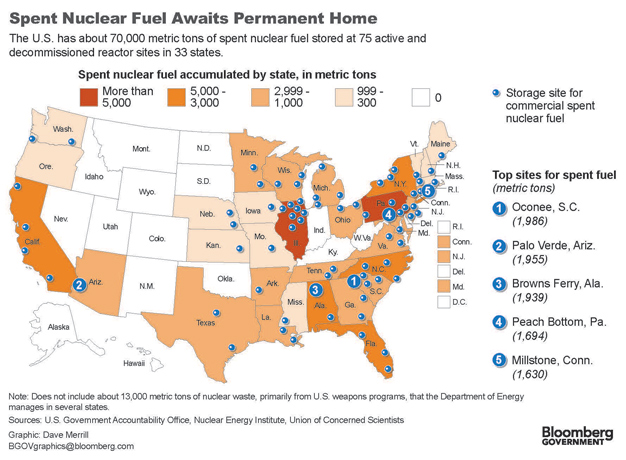
\includegraphics[width=0.80\textwidth]{snf.sites.jpg}
%       \caption{}
    \end{figure}
\end{frame}


\begin{frame}[plain]{}
    \centering\LARGE\textbf{Where else can we put the waste?}
\end{frame}


\addtocounter{framenumber}{-1} 
\begin{frame}{}
    \begin{figure}
        \centering
        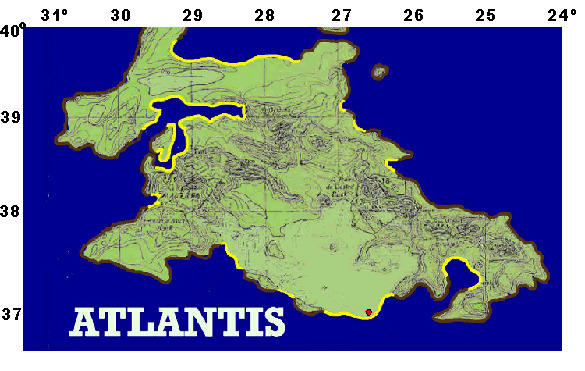
\includegraphics[width=0.85\textwidth]{atlantis.jpg}
%       \caption{}
    \end{figure}
\end{frame}


\begin{frame}{}
    \begin{figure}
        \centering
        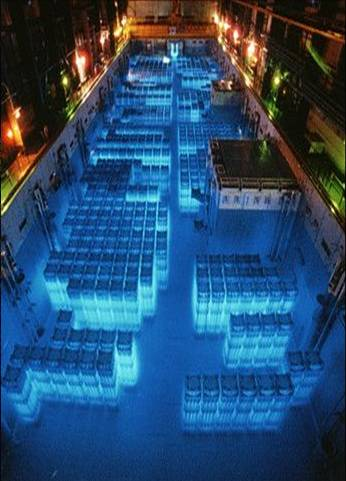
\includegraphics[width=0.60\textwidth]{pool.jpg}
%       \caption{}
    \end{figure}
\end{frame}


\begin{frame}{}
    \begin{figure}
        \centering
        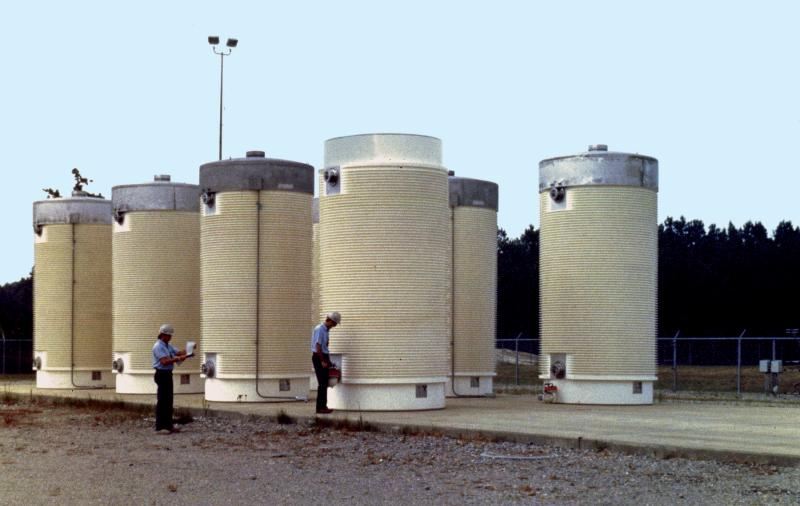
\includegraphics[width=0.85\textwidth]{dry.casks.jpg}
%       \caption{}
    \end{figure}
\end{frame}


\begin{frame}{}
    \begin{figure}
        \centering
        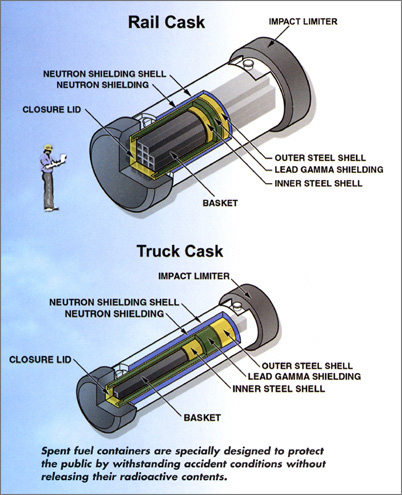
\includegraphics[width=0.45\textwidth]{transport.casks.jpg}
%       \caption{}
    \end{figure}
\end{frame}


\begin{frame}{}
    \begin{figure}
        \centering
        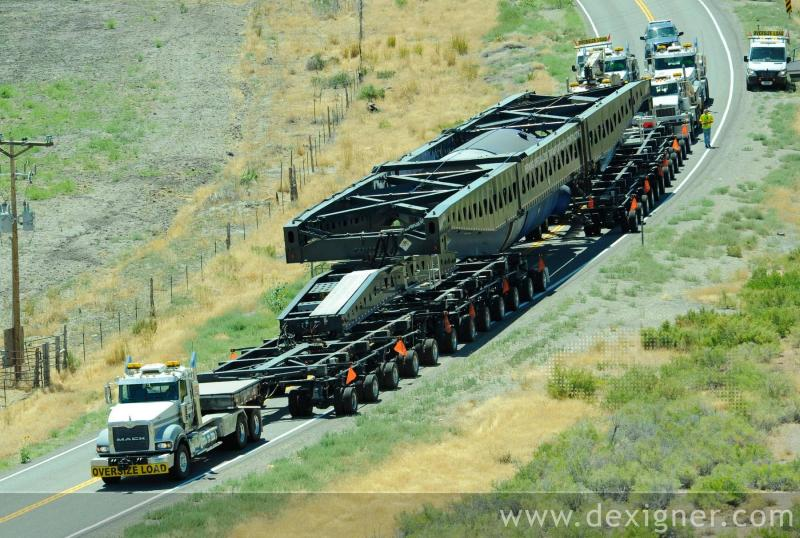
\includegraphics[width=0.85\textwidth]{transport.jpg}
%       \caption{}
    \end{figure}
\end{frame}


\begin{frame}[plain]{}
    \centering\LARGE\textbf{What are the options to dispose of nuclear waste?}
\end{frame}


\addtocounter{framenumber}{-1} 
\begin{frame}{What are the technical limitations of these options?}
    \begin{enumerate}[series=outerlist,topsep=0pt,itemsep=11pt,leftmargin=*,label=(\arabic*)]
        \item[]Near surface engineered storage (\acs{llw})
        \item[]Geologic repository 
        \item[]Deep borehole
        \item[]Ice sheet disposal
        \item[]Sub seabed disposal
        \item[]Spaaaaaacceeeee!
        \item[]Interim aboveground
        \item[]The National Academy of Science judged geologic repositories to be the way waste should be disposed
        \item[]What do you need to know to dispose the waste in the repository?
    \end{enumerate}
\end{frame}


\begin{frame}[plain]{}
    \centering\LARGE\textbf{History}
\end{frame}


\addtocounter{framenumber}{-1} 
\begin{frame}{Waste disposal was thought about from the start}
    \begin{enumerate}[series=outerlist,topsep=0pt,itemsep=21pt,leftmargin=*,label=(\arabic*)]
        \item[]Commercial nuclear development followed Eisenhower's \href{https://youtu.be/2B8R-umE0s0}{Atoms for Peace speech} in 1953
        \item[]Mid-50s -- US made a decision to take naval nuclear reactor technology and apply it to commercial generation of electrical power using civilian owned reactors
        \item[]First commercial nuclear power plant was at Shippingport PA  
        \item[]United States was reprocessing nuclear fuel materials until Carter
        \item[]1955 -- \acf{nas} was asked what to do about waste 
        \item[]1957 -- Disposal in cavities mined in salt is suggested as the possibility promising the most practical immediate solution of the problem
    \end{enumerate}
\end{frame}


\begin{frame}{Waste management is a failure because it was not treated as a social problem}
    \begin{enumerate}[series=outerlist,topsep=0pt,itemsep=21pt,leftmargin=*,label=(\arabic*)]
        \item[]\acs{nas} in 1957 recommended deep disposal in salt 
        \item[]Lyons Kansas was investigated 1957--72 but scrapped due to public opposition
        \item[]\acs{wip} authorized in 1980 and received waste first in 1999
        \item[]\acs{wip} -- \acs{tru} waste from weapons program (1992)
        \item[]1972 -- US abandons repository project at a salt mine in Lyons, KA. Promotes Retrievable Surface Storage Facility as 100-year interim solution
    \end{enumerate}
\end{frame}


\begin{frame}{Waste management lacked a policy direction}
    \begin{enumerate}[series=outerlist,topsep=0pt,itemsep=11pt,leftmargin=*,label=(\arabic*)]
        \item[]1975 -- Geologic disposal adopted as preferred alternative
        \item[]1977 -- Spent fuel reprocessing indefinitely deferred
        \item[]1982 -- \acs{nwa} lays out comprehensive screening process leading to 2 sites in West and East
        \item[]Establishes Nuclear Waste Fund, financed by 0.1 cent/kWh nuclear electricity levy
        \item[]Directs \acs{doe} to begin accepting spent fuel from utilities in 1998
        \item[]That Nuclear Waste Fund has a lot of money now
        \item[]1985 -- President Reagan abandons site search in east
        \item[]1987 -- \acs{nwa} Amendments direct \acs{doe} to focus all site investigation at Yucca Mountain, NV
        \item[]Ended 2nd repository screening activity
    \end{enumerate}
\end{frame}


\begin{frame}{The saga of disposal is far from over}
    \begin{enumerate}[series=outerlist,topsep=0pt,itemsep=21pt,leftmargin=*,label=(\arabic*)]
        \item[]1987 -- Nevada opposed \acs{doe} site characterization and lose in court
        \item[]1998 -- \acs{doe} `Viability Assessment' finds no technical `showstoppers' to proceeding with Yucca Mountain site 
        \item[]1999 -- \acs{doe} issues Draft Environmental Impact Statement concluding that disposal at Yucca Mountain would be safer than leaving the waste where it is
        \item[]2002 -- President approves proceeding with Yucca mountain as nation's first repository
        \item[]Complex national geologic repository site selection process initiated, then abandoned
        \item[]Yucca Mountain picked instead
    \end{enumerate}
\end{frame}


\begin{frame}{\acs{doe} didn't do so well either}
    \begin{enumerate}[series=outerlist,topsep=0pt,itemsep=21pt,leftmargin=*,label=(\arabic*)]
        \item[]\acs{doe} contracts with utilities to take possession of utility spent fuel beginning in 1998, but fails to do so
        \item[]Leaks of high-level radioactive waste from tanks at \acs{doe} sites in Washington and South Carolina
        \item[]Disclosures of contamination and excessive radiation doses to workers throughout \acs{doe} nuclear complex over a period of decades
        \item[]Continuing conflict between federal, state, and local jurisdictions over siting, regulatory issues
        \item[]There is a lot of work to do to restore public trust
    \end{enumerate}
\end{frame}


\begin{frame}{Yucca mountain is not going to be a waste repository}
    \begin{enumerate}[series=outerlist,topsep=0pt,itemsep=21pt,leftmargin=*,label=(\arabic*)]
        \item[]Disposing used fuel is a wasted resource
        \item[]Some will have to be disposed even if we recycle
        \item[]Reprocessing is a sound technology that has half a century of operational history
        \item[]And reduces waste volume
        \item[]Current onsite storage in dry casks is relatively secure
    \end{enumerate}
\end{frame}


\begin{frame}{Consolidated interim storage facilities can offer benefits}
    \begin{enumerate}[series=outerlist,topsep=0pt,itemsep=5pt,leftmargin=*,label=(\arabic*)]
        \item[]\textbf{Pros}
        \item[]Jobs
        \item[]Growth
            \vspace{0.15in}
        \item[]\textbf{Cons}
        \item[]Will become a de facto alternative to disposal
        \item[]\textit{Could write into law that it cannot; give authority to State to make decsion}
        \item[]Will be no easier to site than a repository
        \item[]\textit{That's why they gave us \$2M}
        \item[]Will reduce momentum to develop a repository
        \item[]\textit{Everyone agrees we need one}
            \vspace{0.20in}
        \item[]Back end management needs to be treated as a social problem or there will be no success
    \end{enumerate}
\end{frame}


\begin{frame}[plain]{}
    \centering\LARGE\textbf{\acs{wip} is the first mined repository to receive waste}
\end{frame}


\addtocounter{framenumber}{-1} 
\begin{frame}{\acs{wip} authorized in 1980}
    \begin{enumerate}[topsep=0pt,itemsep=21pt,leftmargin=*,label=(\arabic*)]
        \item[]Received waste first in 1999. From \href{https://twitter.com/nuclear94}{Jeff Terry}!
        \item[]Zero accidents recorded, not counting the moron who lost his badge when we were there
        \item[]\acs{wip} = \acs{tru} waste
        \item[]\href{https://uidaho.pressbooks.pub/nuclearengineering/chapter/doe-waste-disposal-facilities/}{\acs{wip} accident}
    \end{enumerate}
\end{frame}


\begin{frame}{}
    \begin{figure}
        \centering
        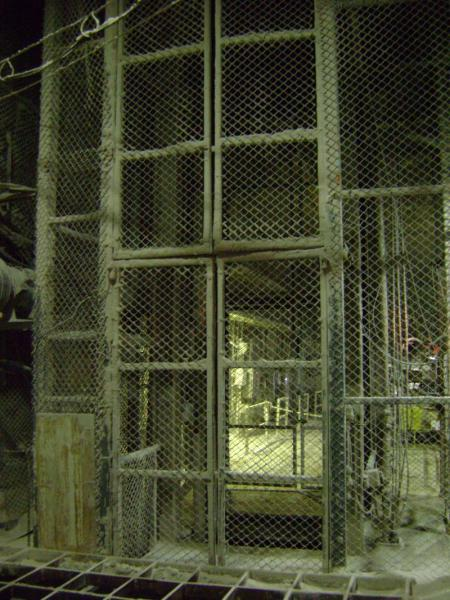
\includegraphics[width=0.45\textwidth]{wipp1.jpg}
%       \caption{}
    \end{figure}
\end{frame}


\begin{frame}{}
    \begin{figure}
        \centering
        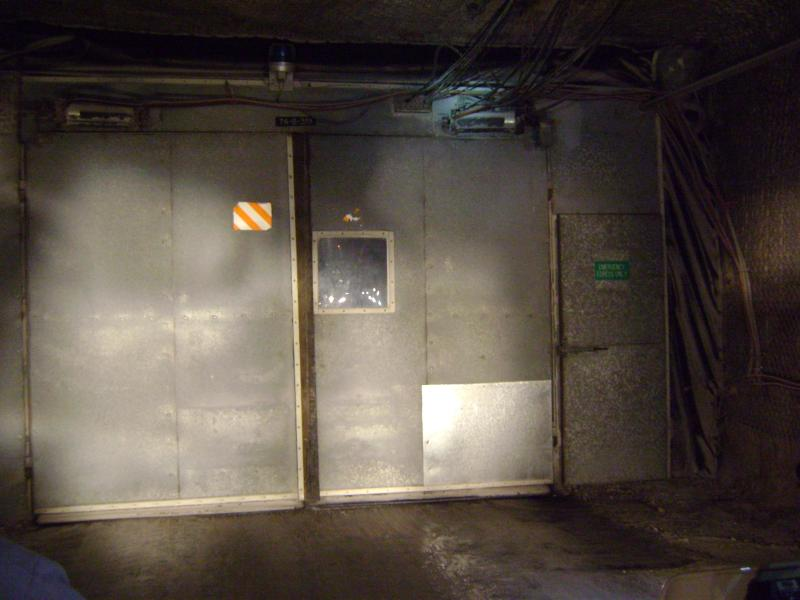
\includegraphics[width=0.75\textwidth]{wipp2.jpg}
%       \caption{}
    \end{figure}
\end{frame}


\begin{frame}{}
    \begin{figure}
        \centering
        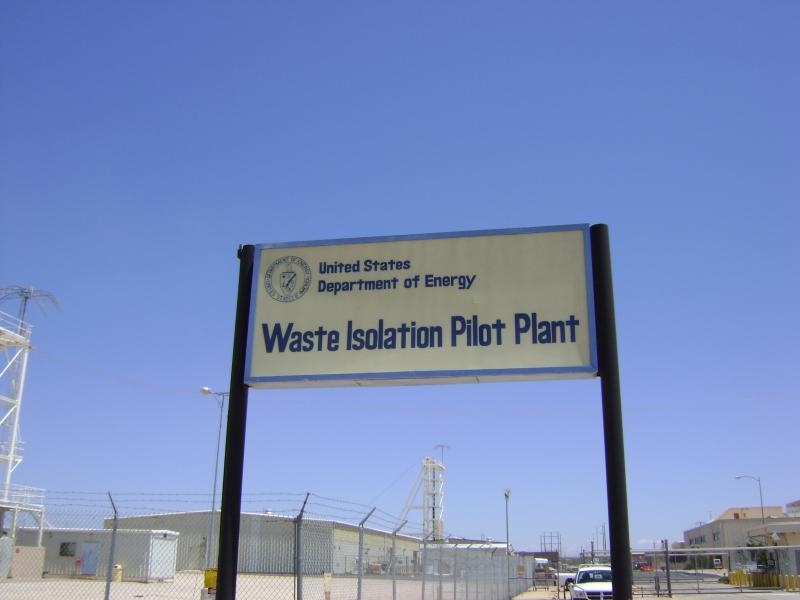
\includegraphics[width=0.75\textwidth]{wipp3.jpg}
%       \caption{}
    \end{figure}
\end{frame}


\begin{frame}{}
    \begin{figure}
        \centering
        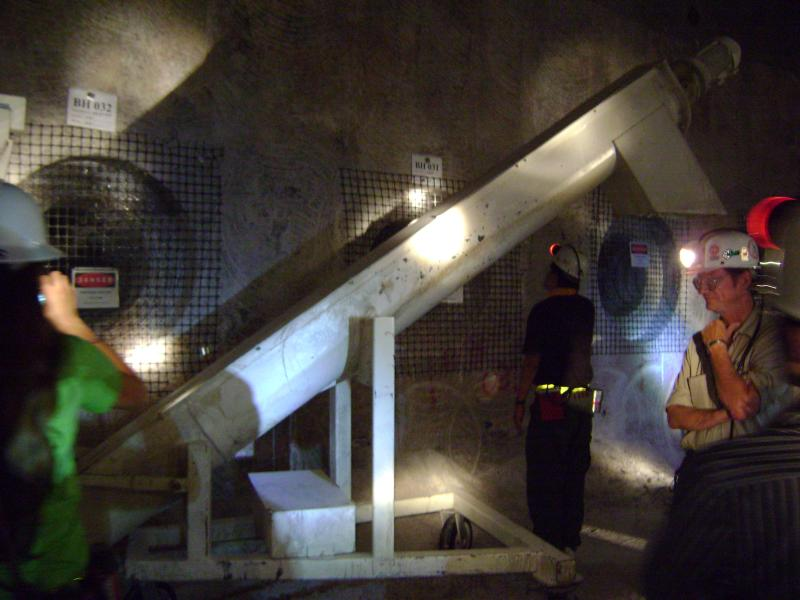
\includegraphics[width=0.75\textwidth]{wipp4.jpg}
%       \caption{}
    \end{figure}
\end{frame}


\begin{frame}{}
    \begin{figure}
        \centering
        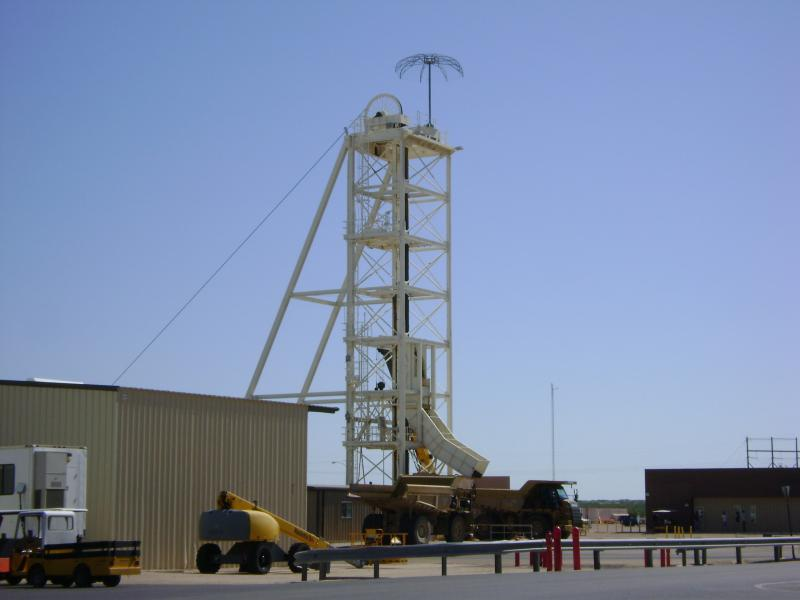
\includegraphics[width=0.75\textwidth]{wipp5.jpg}
%       \caption{}
    \end{figure}
\end{frame}


\begin{frame}{}
    \begin{figure}
        \centering
        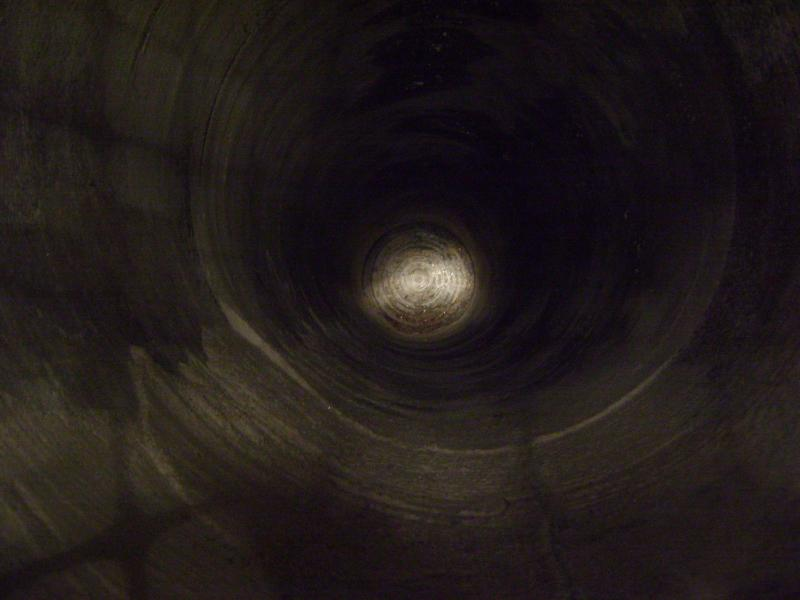
\includegraphics[width=0.75\textwidth]{wipp6.jpg}
%       \caption{}
    \end{figure}
\end{frame}


\begin{frame}{}
    \begin{figure}
        \centering
        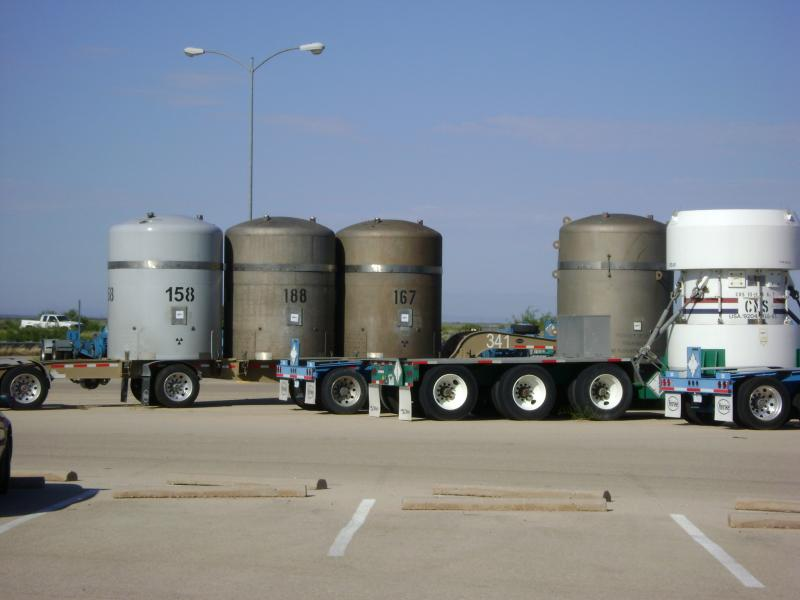
\includegraphics[width=0.75\textwidth]{wipp7.jpg}
%       \caption{}
    \end{figure}
\end{frame}


\begin{frame}{}
    \begin{figure}
        \centering
        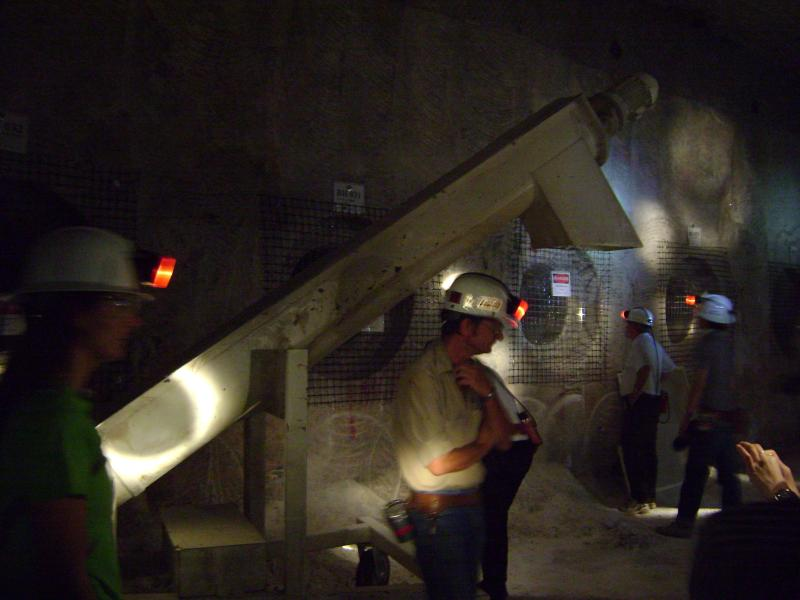
\includegraphics[width=0.75\textwidth]{wipp8.jpg}
%       \caption{}
    \end{figure}
\end{frame}


\begin{frame}{}
    \begin{figure}
        \centering
        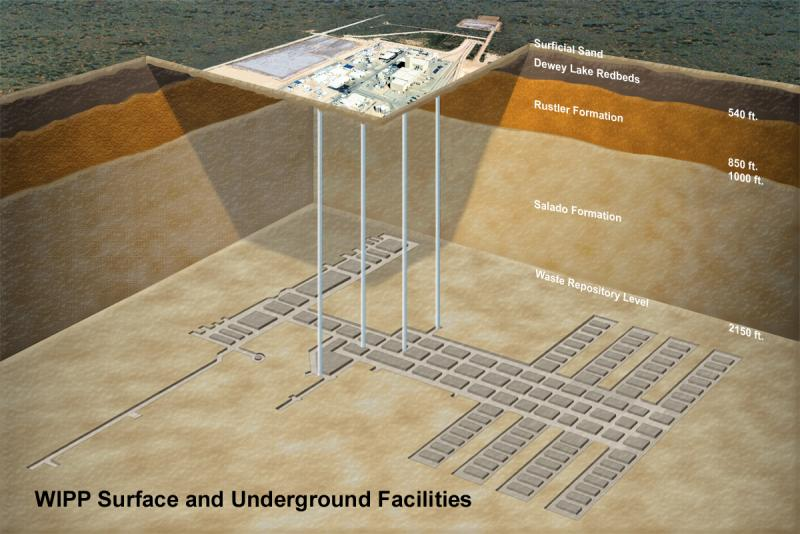
\includegraphics[width=0.85\textwidth]{wipp.jpg}
%       \caption{}
    \end{figure}
\end{frame}


\begin{frame}[plain]{}
    \centering\LARGE\textbf{\acf{nwa}}
\end{frame}


\addtocounter{framenumber}{-1} 
\begin{frame}{\acl{nwa} is the basis for \acs{hlw} management}
    \begin{enumerate}[series=outerlist,topsep=0pt,itemsep=7pt,leftmargin=*,label=(\arabic*)]
        \item[]Established disposal in geologic formation
        \item[]\acs{doe} sites, constructs, operates the repository
        \item[]Sites studied: Hanford, Yucca Mountain, Texas
        \item[]1987 -- \acs{nwa} amended to focus only on Yucca at 70000 \acs{mtm}
        \item[]Supposed to start in 1998
        \item[]A license application was submitted to \acs{nrc} in 2008
        \item[]Obama Administration withdrew any further funding
        \item[]2013 -- Circuit Court ruled for \acs{nrc} to continue safety evaluation
        \item[]2015 -- \href{https://www.nrc.gov/reading-rm/doc-collections/nuregs/staff/sr1949/index.html}{\acs{nrc} Safety Evaluation Report}
        \item[]2016 -- \href{https://www.nrc.gov/waste/hlw-disposal/key-documents.html}{Working Environmental Impact Statement}
    \end{enumerate}
\end{frame}

\begin{frame}[plain]{}
    \centering\LARGE\textbf{But what happens if the license is granted?}
\end{frame}


\begin{frame}[plain]{}
    \centering\LARGE\textbf{How should nuclear facilities be sited?}
\end{frame}


\begin{frame}[plain]{}
    \centering\LARGE\textbf{\acl{brc} on America's nuclear future}
\end{frame}


\addtocounter{framenumber}{-3} 
\begin{frame}{\href{https://uidaho.pressbooks.pub/nuclearengineering/chapter/back-end-of-the-fuel-cycle/}{\acl{brc} was formed to review back-end policy}}
    \begin{enumerate}[series=blue,topsep=0pt,itemsep=21pt,leftmargin=*,label=(\arabic*)]
        \item[]Really, because there wasn't any policy
            \vspace{0.05in}
        \item A new, consent-based approach to siting future nuclear waste management facilities.
        \item A new organization dedicated solely to implementing the waste management program and empowered with the authority and resources to succeed.
        \item Access to the funds nuclear utility ratepayers are providing for the purpose of nuclear waste management.
        \item Prompt efforts to develop one or more geologic disposal facilities.
        \item Prompt efforts to develop one or more consolidated storage facilities.
    \end{enumerate}
\end{frame}


\begin{frame}{\href{https://uidaho.pressbooks.pub/nuclearengineering/chapter/back-end-of-the-fuel-cycle/}{\acl{brc} was formed to review back-end policy}}
    \begin{enumerate}[resume=blue,topsep=0pt,itemsep=21pt,leftmargin=*,label=(\arabic*)]
        \item Prompt efforts to prepare for the eventual large-scale transport of spent nuclear fuel and high-level waste to consolidated storage and disposal facilities when such facilities become available.
        \item Support for continued U.S. innovation in nuclear energy technology and for workforce development.
        \item Active U.S. leadership in international efforts to address safety, waste management, non-proliferation, and
            \vspace{0.05in}
security concerns.
        \item[] Not particularly revolutionary (Peterson), but what other nations are doing around the world
        \item[] The point of the \acs{brc} was to establish consensus
    \end{enumerate}
\end{frame}


\begin{frame}[plain]{}
    \centering\LARGE\textbf{Energy Policy Act}
\end{frame}


\addtocounter{framenumber}{-1} 
\begin{frame}{The Energy Policy Act (1992) set regulatory framework}
    \begin{enumerate}[series=outerlist,topsep=0pt,itemsep=7pt,leftmargin=*,label=(\arabic*)]
        \item[]40CFR197 -- \acs{epa} radioactivity releases
        \item[]Individual protection standard   
        \item[]Groundwater protection standard   
        \item[]Human intrusion standard  
        \item[]No greater than 15 mrem per year for the maximally-exposed individual during first 10000 years
        \item[](National average background is 300 mrem)
        \item[]Parameters describing human activity and behavior `will remain as there are today'
        \item[]\acs{nrc} verifies compliance with performance assessments, risk-informed approach
        \item[]10CFR63 -- Construction, operation, closure, 15 mrem limit
        \item[]1995 -- \acs{nas} review
        \item[]Extended time frame of peak risk to (of adverse health effects) \textit{1 million years} 
    \end{enumerate}
\end{frame}


\begin{frame}{}
    \begin{figure}
        \centering
        
\includegraphics[width=0.75\textwidth]{doctor.evil.jpg}
%        \caption{}
    \end{figure}
\end{frame}


\begin{frame}{The Energy Policy Act (1992) had \acs{nas} to review the whole issue of disposal}
    \begin{enumerate}[series=outerlist,topsep=0pt,itemsep=21pt,leftmargin=*,label=(\arabic*)]
        \item[]Can scientifically justifiable analyses of repository behavior over many thousands of years in the future be made?
        \item[]Recommended the use of a standard that sets a limit on the risk to individuals of adverse
health effects from releases from the repository is recommended
        \item[]Extension of time frame from 10000 to a million years
        \item[]Based on long term stability of the geologic environment
    \end{enumerate}
\end{frame}


\begin{frame}[plain]{}
    \centering\LARGE\textbf{Functional components and technical basis}
\end{frame}


\addtocounter{framenumber}{-1} 
\begin{frame}{What are the functional components for repository performance?}
    \begin{enumerate}[series=outerlist,topsep=0pt,itemsep=21pt,leftmargin=*,label=(\arabic*)]
        \item[]Waste cannot be released to biosphere at unacceptable concentrations
        \item[]Waste must be removed and isolated from catastrophic natural events or human activity
        \item[]Must be able to use current technology and engineering at reasonable cost
        \item[]Widely acceptable performance assessment modeling
        \item[]\href{https://youtu.be/ayLxB9fV2y4}{Into Eternity}
    \end{enumerate}
\end{frame}


\begin{frame}{Waste is inevitably going to get out}
    \begin{enumerate}[series=outerlist,topsep=0pt,itemsep=15pt,leftmargin=*,label=(\arabic*)]
        \item[]Contain (isolate) waste as long as possible
        \item[]Maintain engineered barrier system for $10^5 \; y$
        \item[]Physically isolated in a matrix/waste form (vitrified glass)
        \item[]Then put that in a canister
        \item[]During containment, we rely on decay to wipe out most of the radionuclides (at least 300 years)
        \item[]Which are the two most important in the near term?
        \item[]Engineers generally agree that maintaining integrity to about 1000 years is possible
        \item[]When waste does get out, we want controlled release and dispersal based on natural processes
    \end{enumerate}
\end{frame}


\begin{frame}{Controlled release = multi barrier concept}
    \begin{enumerate}[series=outerlist,topsep=0pt,itemsep=11pt,leftmargin=*,label=(\arabic*)]
        \item[]Multi barrier concept aka defense in depth
        \item[]Very common approach in all fields of risk assessment
        \item[]Redundancy and diversity
        \item[]Common examples of this?
        \item[]For the repository, a series of engineered and natural barriers
        \item[]Multi barrier is an holistic concept
        \item[]Act in concert
        \item[]Delay and decay
        \item[]Host rock
        \item[]Groundwater
    \end{enumerate}
\end{frame}


\begin{frame}[t]{}
    \begin{enumerate}[series=outerlist,topsep=0pt,itemsep=21pt,leftmargin=*,label=(\arabic*)]
        \item[]Waste form
        \item[]Canister
        \item[]Backfill
        \item[]Should not have common failure modes  
    \end{enumerate}
\end{frame}


\begin{frame}{Delay and decay means contain and extend transport}
    \begin{enumerate}[series=outerlist,topsep=0pt,itemsep=15pt,leftmargin=*,label=(\arabic*)]
        \item[]If containment time is $10 \times$ greater than half life, then all set
        \item[]Containment for $300 - 1000 \; y$ is effective in eliminating Co-60, Sr-90, Cs-137
        \item[]Repository will also approach ambient temperature by this time
        \item[]Non sorbing radionuclides are problematic though
        \item[]Similarly if transport time is greater than $10 \times$, also set
        \item[]Want diffusion to dominate over advection
        \item[]How can this be achieved?
    \end{enumerate}
\end{frame}


\begin{frame}{How are multi barriers applied to repository design?}
    \begin{enumerate}[series=outerlist,topsep=0pt,itemsep=1pt,leftmargin=*,label=(\arabic*)]
        \item[]Waste package is the waste form and canister
        \item[]Resistant to leaching by groundwater, chemically and physically
            \vspace{0.15in}
        \item[]\textbf{Backfill}
        \item[]Placed around everything once its put in there
        \item[]Inhibits groundwater movement
        \item[]Chemically inhibitive; clay is negatively charged, radionuclides are postive
            \vspace{0.15in}
        \item[]\textbf{Geologic structure}
        \item[]Isolates waste from humans 
        \item[]Chemically, mechanically stable
        \item[]Prevents/restricts circulating groundwater
        \item[]Slows releases to biosphere
    \end{enumerate}
\end{frame}


\begin{frame}{}
    \begin{figure}
        \centering
        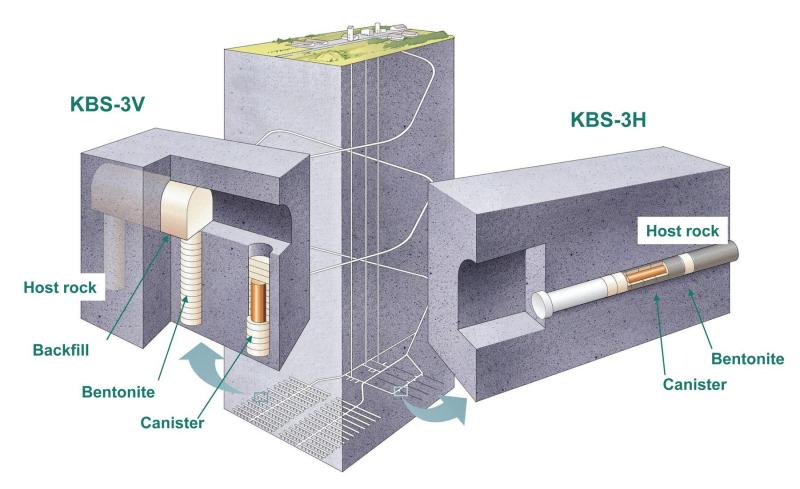
\includegraphics[width=0.85\textwidth]{kbs.jpg}
%       \caption{}
    \end{figure}
\end{frame}


\begin{frame}{}
    \begin{figure}
        \centering
        
\includegraphics[width=0.70\textwidth]{repository.jpg}
%       \caption{}
    \end{figure}
\end{frame}


\begin{frame}{Across the world, there are different repository concepts}
    \begin{enumerate}[series=outerlist,topsep=0pt,itemsep=18pt,leftmargin=*,label=(\arabic*)]
        \item[]Switzerland -- granite
        \item[]France -- clay
        \item[]Sweden -- granite
        \item[]Belguim -- clay
        \item[]Finland -- granite 
        \item[]United Kingdom -- granite
        \item[]Japan -- granite
        \item[]Korea -- granite
    \end{enumerate}
\end{frame}


\begin{frame}{Each country legally responsible for waste management and disposal}
    \begin{enumerate}[series=outerlist,topsep=0pt,itemsep=21pt,leftmargin=*,label=(\arabic*)]
        \item[]All saturated
        \item[]Most all have the quasi-federal companies
        \item[]Do we have similar formations in the USA?
        \item[]What is the best formation?
    \end{enumerate}
\end{frame}


\begin{frame}{Siting is a decades long process}
    \begin{enumerate}[series=outerlist,topsep=0pt,itemsep=1pt,leftmargin=*,label=(\arabic*)]
        \item[]\textbf{Before you even start}
        \item[]Assuming a locality volunteers
        \item[]Public acceptance, both local and national
        \item[]In USA, we have extra layer of state government
            \vspace{0.10in}
        \item[]\textbf{Geology}
        \item[]Structurally stable geological block 
        \item[]Not near a tectonic boundary
        \item[]Avoid faults along which rupture could occur
        \item[]Avoid areas with abnormally high geothermal
        \item[]Gradients or with evidence of relatively recent volcanic activity
        \item[]Mechanical properties should assure stability during operation
        \item[]Competing land use like parks, oil, gas
        \item[]Transportation requirements
    \end{enumerate}
\end{frame}


\begin{frame}[t]{}
    \begin{enumerate}[series=outerlist,topsep=0pt,itemsep=1pt,leftmargin=*,label=(\arabic*)]
        \item[]\textbf{Hydrology}
        \item[]Fluid transport should not move hazardous material to the biosphere in amounts and rates above prescribed limits
        \item[]Low permeability
        \item[]Low flow
        \item[]System should be capable of being sealed when the repository is closed
        \item[]Geological record should support predictions favorable for long-term hydrological isolation of the repository site in a perturbed geological environment
        \item[]Most places in Europe are not like that
    \end{enumerate}
\end{frame}


\begin{frame}[t]{}
    \begin{enumerate}[series=outerlist,topsep=0pt,itemsep=1pt,leftmargin=*,label=(\arabic*)]
        \item[]\textbf{Geochemistry}
        \item[]Heat, radiation should not produce physical, chemical reactions in the rock that would compromise containment
        \item[]Low oxygen
        \item[]Low redox potential ($Eh$)
        \item[]Near neutral $pH$
        \item[]Low concentrations of complexing anions and organics
        \item[]Conditions should minimize the rate of dissolution of the waste form (typically reducing)
        \item[]Water in the repository should not react to increase permeability
        \item[]Limit mobility of radionuclides and delay or prevent their migration to the biosphere
        \item[]No area with record of resource extraction
        \item[]What type of places can you actually site?
    \end{enumerate}
\end{frame}


\begin{frame}[plain]{}
    \centering\LARGE\textbf{How long is long term?}
\end{frame}


\begin{frame}[plain]{}
    \centering\LARGE\textbf{What are the oldest human constructed formations?}
\end{frame}


\addtocounter{framenumber}{-2} 
\begin{frame}{Multiple barriers are engineered to provide defense in depth}
    \begin{enumerate}[series=outerlist,topsep=0pt,itemsep=21pt,leftmargin=*,label=(\arabic*)]
        \item[]This is the basis for any risk management approach
        \item[]What actually happens in the repository?
        \item[]The whole point is that after everything gets put in you close the repository and walk away
        \item[]It is supposed to function on its own
        \item[]Why?
        \item[]Limit exposures in the long term
        \item[]Compliance demonstrated by the performance assessment
    \end{enumerate}
\end{frame}


\begin{frame}{Know your materials science}
    \begin{enumerate}[series=outerlist,topsep=0pt,itemsep=3pt,leftmargin=*,label=(\arabic*)]
        \item[]Corrosion resistant metals with inert oxide surface layer
        \item[]Low rate of corrosion in water
        \item[]Advanced materials
        \item[]New alloy made for Yucca Mountain casks
        \item[]Compatible with repository environment
        \item[]Buffer assures slow diffusion and high sorption
        \item[]Diffusion dominated transport
        \item[]Long transit time, delay and decay
        \item[]Constrain corrosion rate
        \item[]Seal fractures due to construction
        \item[]Saturated repositories use bentonite
        \item[]Each has different chemical make up $Na^+,Ca^{++}$ interlayer ions
        \item[]For unsaturated conditions, use sand over gravel
    \end{enumerate}
\end{frame}


\begin{frame}{Other processes to consider}
    \begin{enumerate}[series=outerlist,topsep=0pt,itemsep=21pt,leftmargin=*,label=(\arabic*)]
        \item[]Thermal management
        \item[]Subcritical configuration
        \item[]Waste form dissolution
        \item[]Diffusion
        \item[]Solubility
        \item[]Corrosion
    \end{enumerate}
\end{frame}


\begin{frame}{What is each barrier expected to do?}
    \begin{enumerate}[series=outerlist,topsep=0pt,itemsep=1pt,leftmargin=*,label=(\arabic*)]
        \item[]\textbf{Geologic formation}
        \item[]isolate the \acs{ebs} from biosphere
        \item[]geomechanical stability
        \item[]favorable geochemistry
        \item[]limit groundwater flow
            \vspace{0.10in}
        \item[]\textbf{Backfill}
        \item[]contain \acs{ebs}
        \item[]limit fast release pathways
        \item[]mechanical stability of tunnels
    \end{enumerate}
\end{frame}


\begin{frame}[t]{}
    \begin{enumerate}[series=outerlist,topsep=0pt,itemsep=1pt,leftmargin=*,label=(\arabic*)]
        \item[]\textbf{Buffer}
        \item[]diffusive dominated transport 
        \item[]isolate canister from formation
        \item[]conduct heat
            \vspace{0.10in}
        \item[]\textbf{Canister}
        \item[]isolate waste for long time period
        \item[]mechanical stability
        \item[]conduct heat
    \end{enumerate}
\end{frame}


\begin{frame}{We want to draw on accepted methods and design bottom-up}
    \begin{enumerate}[series=outerlist,topsep=0pt,itemsep=21pt,leftmargin=*,label=(\arabic*)]
        \item[]Readily available technologies
        \item[]Retrievability
        \item[]Based on well accepted models
        \item[]Risk informed approach
        \item[]Environmental modeling
        \item[]We want to use what we know well so we are confident in results
    \end{enumerate}
\end{frame}


\begin{frame}{Waste must be contained `as long as necessary'}
    \begin{enumerate}[series=outerlist,topsep=0pt,itemsep=15pt,leftmargin=*,label=(\arabic*)]
        \item[]This depends on making a robust waste form 
        \item[]Borosilicate glass or ceramic matrix
        \item[]`Long enough' so most radionuclides decay away $\approx 1000 \; y$
        \item[]Significant heat comes from $^{137}Cs$ and $^{90}Sr$
        \item[]Actinides like Pu, Cm, etc., are long lived, but low radioactivity
        \item[]They are really toxic though because they are heavy metals
        \item[]Oxidation state of Np makes it very mobile
        \item[]Iodine is a negative ion so also very mobile
    \end{enumerate}
\end{frame}


\begin{frame}{When there is release, it must be diluted and dispersed}
    \begin{enumerate}[series=outerlist,topsep=0pt,itemsep=21pt,leftmargin=*,label=(\arabic*)]
        \item[]Clay can trap the radionuclides ($\pm$ charges)
        \item[]A lot of water can dilute the contaminant plume
    \end{enumerate}
\end{frame}


\begin{frame}{The multi-barrier concept is a series of engineered and natural barriers to delay release}
    \begin{enumerate}[series=outerlist,topsep=0pt,itemsep=21pt,leftmargin=*,label=(\arabic*)]
        \item[]No common failure modes
        \item[]Waste form -- dissolution and solubility modeling
        \item[]Waste container
        \item[]Buffer -- Diffusion of radionuclides, sorption
        \item[]Backfill -- Diffusion of radionuclides, sorption
        \item[]Geological structure -- requires decades long studies
        \item[]Diffusion, dispersion, advection, sorption modeling, ion exchange
    \end{enumerate}
\end{frame}


\begin{frame}{}
    \begin{figure}
        \centering
        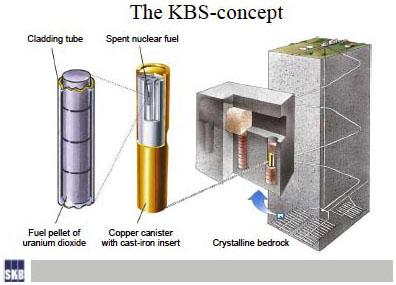
\includegraphics[width=0.85\textwidth]{kbs.canister.jpg}
%       \caption{}
    \end{figure}
\end{frame}


\begin{frame}[plain]{}
    \centering\LARGE\textbf{Yucca Mountain}\\
    \centering\LARGE\textbf{\acf{tpa}}
\end{frame}


\addtocounter{framenumber}{-1} 
\begin{frame}{The \acs{tpa} models all possible scenarios for release }
    \begin{enumerate}[resume=blue,topsep=0pt,itemsep=21pt,leftmargin=*,label=(\arabic*)]
        \item[]\href{https://www.osti.gov/servlets/purl/1142603}{Summary by Peter Swift}
    \end{enumerate}
\end{frame}


\begin{frame}{}
    \begin{figure}
        \centering
        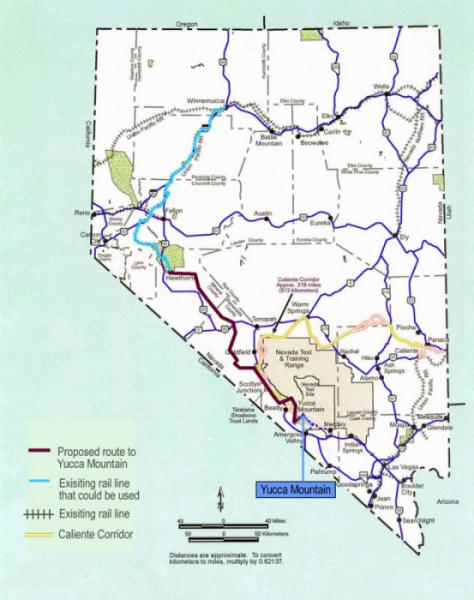
\includegraphics[width=0.45\textwidth]{nevada.map.jpg}
%       \caption{}
    \end{figure}
\end{frame}


\begin{frame}{}
    \begin{figure}
        \centering
        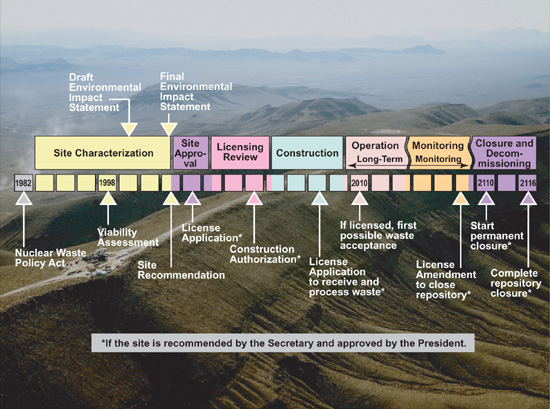
\includegraphics[width=0.75\textwidth]{timeline.jpg}
%       \caption{}
    \end{figure}
\end{frame}


\begin{frame}{Aside -- \acs{doe} \& \acs{hlw} is stored at Hanford and Savannah river}
    \begin{enumerate}[series=outerlist,topsep=0pt,itemsep=21pt,leftmargin=*,label=(\arabic*)]
        \item[]Really made a mess of it
        \item[]Tanks have leaked into soil
        \item[]People are worried about toxicity in Columbia River
        \item[]First large scale plutonium production reactor
        \item[]Legacy of the cold war
    \end{enumerate}
\end{frame}


\begin{frame}{Yucca mountain has a unique geology compared other repository concepts}
    \begin{enumerate}[series=outerlist,topsep=0pt,itemsep=18pt,leftmargin=*,label=(\arabic*)]
        \item[]100 miles northwest of Las Vegas (the wiseguys not happy)
        \item[]Volcanic tuff
        \item[]Layers of consolidated, compacted ashfalls from volcanic eruptions occurring more than 10 million years ago 
        \item[]Underlying the tuff is sedimentary carbonate rock
        \item[]Repository horizon in unsaturated zone, about 300 meters below the surface, and 300-500 meters above the water table
        \item[]Two major aquifers in the saturated zone below Yucca Mountain, one in tuff, one in carbonate rock
    \end{enumerate}
\end{frame}


\begin{frame}{Which leads to different operating concepts}
    \begin{enumerate}[series=outerlist,topsep=0pt,itemsep=18pt,leftmargin=*,label=(\arabic*)]
        \item[]Yucca Mountain would remain open with active ventilation for at least a hundred years
        \item[]This allows a significant fraction of decay heat to go to the atmosphere and reduces peak post closure temperatures
        \item[]That's easier to do because the repository is not saturated
        \item[]Unsaturated zone design allows long term monitoring and, if necessary, retrieval, modification or repair
    \end{enumerate}
\end{frame}


\begin{frame}{The design is also different than the other repositories}
    \begin{figure}
        \centering
        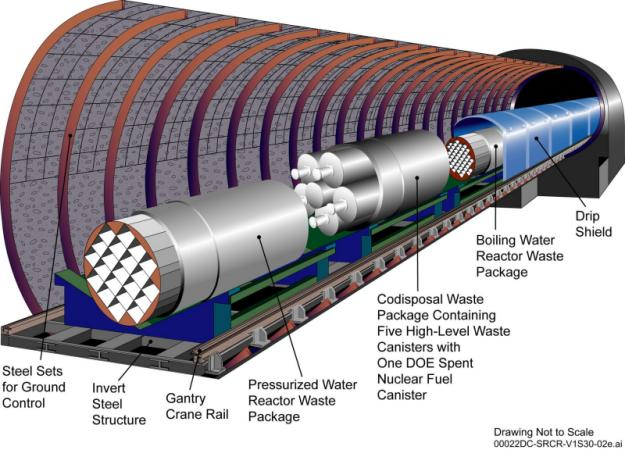
\includegraphics[width=0.75\textwidth]{yucca.waste.jpg}
%       \caption{}
    \end{figure}
\end{frame}


\begin{frame}{}
    \begin{figure}
        \centering
        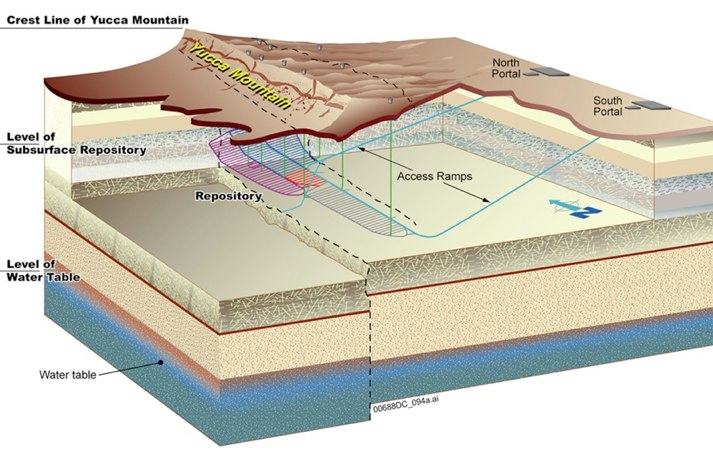
\includegraphics[width=0.75\textwidth]{yucca.geology.jpg}
%       \caption{}
    \end{figure}
\end{frame}


\begin{frame}[plain]{}
    \centering\LARGE\textbf{What are the failure modes for the repository?}
\end{frame}


\begin{frame}[plain]{}
    \centering\Large\textbf{What is the world going to look like in $10^3, \; 10^4, \; 10^5$ years?}
\end{frame}


\addtocounter{framenumber}{-2} 
\begin{frame}{}
    \begin{figure}
        \centering
        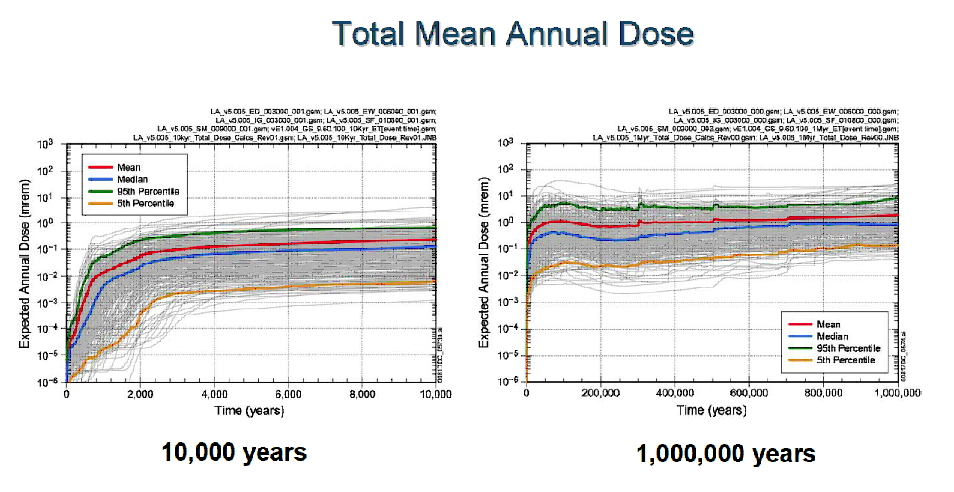
\includegraphics[width=0.95\textwidth]{yucca.mountain.jpg}
%        \caption{}
    \end{figure}
\end{frame}


\begin{frame}{What are the failure modes for the repository?}
    \begin{enumerate}[series=outerlist,topsep=0pt,itemsep=21pt,leftmargin=*,label=(\arabic*)]
        \item[]Degradation over time
        \item[]Natural and engineered barriers
        \item[]Dissolution and transport of radionuclides in groundwater
        \item[]Tectonic processes -- folding, faulting, magmatic intrusions, volcanism
        \item[]Erosion -- wind, water, glaciation
        \item[]Breaching of barriers by human activity
        \item[]Aliens
    \end{enumerate}
\end{frame}


\begin{frame}{The performance assessment predicts how the repository will respond}
    \begin{enumerate}[series=outerlist,topsep=0pt,itemsep=11pt,leftmargin=*,label=(\arabic*)]
        \item[]Rate of inflow of groundwater into the repository
        \item[]Hydrology current, long-term, fracturing, faulting, thermal stresses in host rock
        \item[]Rate of corrosion of canister, other barriers, and primary waste form
        \item[]Temperature, oxidation/reduction conditions, materials properties of waste package
        \item[]Yucca mountain is an oxidizing environment, different than world standards
        \item[]Radionuclide transport in groundwater, sorption on rock surfaces, actinide chemistry
        \item[]Biosphere transport in potable water supplies, irrigation water, demography dose 
        \item[]How safe is safe enough?
        \item[]Assumptions about future human activities and lifestyles
        \item[]How far into the future is it reasonable to project disposal system performance?
    \end{enumerate}
\end{frame}


\begin{frame}{Who needs to know the repository is safe?}
    \begin{enumerate}[series=outerlist,topsep=0pt,itemsep=11pt,leftmargin=*,label=(\arabic*)]
        \item[]\textbf{Implementer} -- to have confidence to present and defend a license application
        \item[]\textbf{Regulator} -- to be able to license the repository
        \item[]\textbf{Elected Representatives} -- to be justified in taking a decision to proceed
        \item[]\textbf{Public} -- to have confidence in and accept the whole process
        \item[]The relative roles and participation is going to vary with location and people
        \item[]Perception of safety is different for the public
        \item[]\acs{ala} v precautionary principle
        \item[]Defining risk for specific context
        \item[]Risk communication (resiliency) is extremely difficult
    \end{enumerate}
\end{frame}


\begin{frame}{Public trust must be cultivated}
    \begin{enumerate}[series=outerlist,topsep=0pt,itemsep=21pt,leftmargin=*,label=(\arabic*)]
        \item[]The arguments they hear should be based upon what they can understand and relate to their experience
        \item[]They need to see relevant information and that nothing is being hidden
        \item[]Really public have different priorities and concerns than what experts think
        \item[]Experts need to develop social science literacy
        \item[]Consent-based siting should be social science led
    \end{enumerate}
\end{frame}


\begin{frame}{Safety is dependent on an independent regulator}
    \begin{enumerate}[series=outerlist,topsep=0pt,itemsep=11pt,leftmargin=*,label=(\arabic*)]
        \item[]Assure that post-closure safety meets international accepted standards
        \item[]Confirm that uncertainty has been properly considered
        \item[]Are system models complete and valid?
        \item[]Are appropriate parameter values and ranges identified?
        \item[]Are analyses conducted to identify processes \& parameters most important to safety?
        \item[]Are `what if\ldots' scenarios analyzed?
        \item[]Conduct independent review and assessment of safety
        \item[]Require Implementer to present multiple lines of evidence
        \item[]Public comment
    \end{enumerate}
\end{frame}


\begin{frame}{What evidence could the operator provide?}
    \begin{enumerate}[series=outerlist,topsep=0pt,itemsep=21pt,leftmargin=*,label=(\arabic*)]
        \item[]There is no data cohort for a repository
        \item[]Uncertainties in extrapolating conditions today into the future
        \item[]Increased confidence from defense-in-depth technical arguments
        \item[]Matching of time scales between repository assessment and natural/archaeological analogues
        \item[]Calculated doses can have relatively large uncertainties
        \item[]Verification/validation of safety assessment codes 
        \item[]Analyze an analogue using the same component models
    \end{enumerate}
\end{frame}


\begin{frame}{}
    \begin{figure}
        \centering
        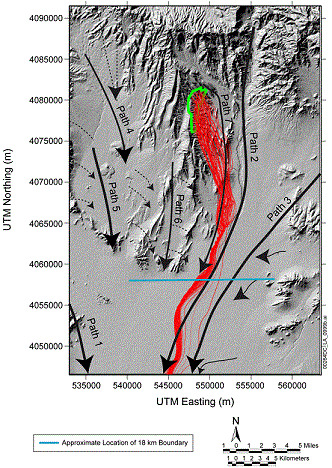
\includegraphics[width=0.40\textwidth]{groundwater.flow.jpg}
%       \caption{}
    \end{figure}
\end{frame}


\begin{frame}[plain]{}
    \centering\Large\textbf{Technical design of a repository}
\end{frame}


\addtocounter{framenumber}{-1} 
\begin{frame}{What is there to design for the repository?}
    \begin{enumerate}[series=outerlist,topsep=0pt,itemsep=7pt,leftmargin=*,label=(\arabic*)]
        \item[]Canister spacing -- Why?
        \item[]\acs{hlw}is vitrified (not the used fuel) to a glass waste form
        \item[]\acs{hlw} producers required to have Waste Acceptance Program 
        \item[]Drift spacing -- $81 \; m$
        \item[]Mid-pillar peak temperature of $96^oC$
        \item[]Waste package spacing -- $0.1 \; m$
        \item[]Average emplacement drift line load -- $1.45 \; kW/m$
        \item[]Maximum waste package thermal output -- $18.0 kW$
        \item[]Ventilation flow rate -- $15 \; m^3/s$
        \item[]23 years of waste emplacement followed by 50 years of forced ventilation following emplacement of the last waste package
        \item[]Design of the process and the waste form determines thermal load
    \end{enumerate}
\end{frame}


\begin{frame}{Specifications developed by \acs{doe} Environmental Management for the \acs{hlw} form producers as their Waste Acceptance Program}
    \begin{enumerate}[series=outerlist,topsep=0pt,itemsep=7pt,leftmargin=*,label=(\arabic*)]
        \item[]\textbf{Chemical}
        \item[]Waste form -- 20--40 w/o waste oxides, 35--65 w/o silica, 5--10 w/o boron oxide, 10--20 w/o alkali oxides, and other oxide constituents
        \item[]Chemical composition, crystalline phases expected to be present, and the amount of each crystalline phase should be identified
        \item[]Oxide composition of waste form should be reported, including all elements (excluding oxygen) present in concentrations greater than 0.5\% of the glass
    \end{enumerate}
\end{frame}


\begin{frame}[t]{}
    \begin{enumerate}[series=outerlist,topsep=0pt,itemsep=7pt,leftmargin=*,label=(\arabic*)]
        \item[]\textbf{Radionuclide inventory}
        \item[]Half-lives longer than 10 years that are or will be present in concentrations greater than 0.05\% of total are, be, 0.05\% radioactive inventory shall be reported (indexed to the year 2015 and 3115)
        \item[]Total quantities of individual radionuclides to be shipped to the repository
        \item[]Upper limit of these radionuclides for any canistered waste form calculated
        \item[]Average calculated radionuclide inventory per canister
        \item[]Quality control by comparing to Environmental Assessment Benchmark Glass
        \item[]At time of shipment, temperature has to be below $400^oC$
        \item[]Rules for nonradionuclide hazardous waste
        \item[]For fissile content for all the isotopes
    \end{enumerate}
\end{frame}


\begin{frame}{There are multi dimensional constraints on canister loading}
    \begin{enumerate}[series=outerlist,topsep=0pt,itemsep=21pt,leftmargin=*,label=(\arabic*)]
        \item[]Waste composition in canister
        \item[]Number of canisters
        \item[]Materials
        \item[]Canister dimensions
        \item[]Radiation
        \item[]Repository conditions
        \item[]Storage conditions
            \vspace{0.15in}
        \item[]Need a systematic way to optimize constraints
    \end{enumerate}
\end{frame}


\begin{frame}[plain]{}
    \centering\Large\textbf{Linear programming}
\end{frame}


\addtocounter{framenumber}{-1} 
\begin{frame}{Linear programming is a good modeling approach}
    \begin{enumerate}[series=outerlist,topsep=0pt,itemsep=1pt,leftmargin=*,label=(\arabic*)]
        \item[]Waste composition --
    \end{enumerate}

    \vspace*{\fill}

    \begin{equation}
        \Large
        \overline{N}_W = [x_{W_1}, \ldots, x_{W_i}, \ldots, x_{W_n}]
    \end{equation}

    \vspace*{\fill}

    \begin{enumerate}[series=outerlist,topsep=0pt,itemsep=1pt,leftmargin=*,label=(\arabic*)]
        \item[]Glass composition --
    \end{enumerate}

    \vspace*{\fill}

    \begin{equation}
        \Large
        \overline{N}_G = [x_{G_1}, \ldots, x_{G_i}, \ldots, x_{G_n}]
    \end{equation}

    \vspace*{\fill}

    \begin{enumerate}[series=outerlist,topsep=0pt,itemsep=1pt,leftmargin=*,label=(\arabic*)]
        \item[]Total mass of solid waste --
    \end{enumerate}

    \vspace*{\fill}

    \begin{equation}
        \Large
        M_S = M_W + M_G
    \end{equation}

    \vspace*{\fill}

    \begin{enumerate}[series=outerlist,topsep=0pt,itemsep=1pt,leftmargin=*,label=(\arabic*)]
        \item[]Solid form composition --
    \end{enumerate}

    \vspace*{\fill}

    \begin{equation}
        \Large
        \overline{N}_S = \theta\overline{N}_W + (1 - \theta)\overline{N}_G
    \end{equation}

    \begin{equation}
        \Large
        \theta \equiv \frac{M_W}{M_S}
    \end{equation}
\end{frame}


\begin{frame}{Linear programming is widely used for optimization}
    \begin{enumerate}[series=outerlist,topsep=0pt,itemsep=1pt,leftmargin=*,label=(\arabic*)]
        \item[]Optimize an objective function --
    \end{enumerate}

    \vspace*{\fill}

    \begin{equation}
        \LARGE
        max(f) = \underline{c} \underline{x}
    \end{equation}

    \vspace*{\fill}

    \begin{enumerate}[series=outerlist,topsep=0pt,itemsep=1pt,leftmargin=*,label=(\arabic*)]
        \item[]Where $\underline{x}$ is constrained --
    \end{enumerate}

    \vspace*{\fill}

    \begin{equation}
        \LARGE
        \underline{\underline{A}} \; \underline{x} \leq \underline{b}
    \end{equation}

    \vspace*{\fill}

    \begin{enumerate}[series=outerlist,topsep=0pt,itemsep=5pt,leftmargin=*,label=(\arabic*)]
        \item[]$c \equiv$ row vector of coefficients of objective function
        \item[]$x \equiv$ column vector of independent variables
        \item[]$A \equiv$ matrix of coefficients of constraint inequalities
        \item[]$b \equiv$ column vector of RHS of constraint inequalities
        \item[]$A$ and $b$ would be based on the regulations for the waste form/canister
    \end{enumerate}
\end{frame}


\begin{frame}[plain]{}
    \centering\Large\textbf{Linear programming example}
\end{frame}


\addtocounter{framenumber}{-1} 
\begin{frame}{Maximize profit for a gas processing plant}
    \begin{enumerate}[series=outerlist,topsep=0pt,itemsep=21pt,leftmargin=*,label=(\arabic*)]
        \item[]A gas processing plant receives a fixed amount of raw gas each week
        \item[]Either regular or premium quality is processed, but only one grade at a time
        \item[]The plant is open 80 hours per week
        \item[]Decision variables are quantity of regular gas and premium gas produced per week
        \item[]Objective function is to maximize profit under given constraints
    \end{enumerate}
\end{frame}


\begin{frame}{}
    \setlength{\arrayrulewidth}{0.3mm}
    \begin{longtable}{l|c|c}
        \caption{Gas processing constraints}
        \label{tab-gas-processing}
        \\
%        \hline
        \textbf{Constraint}
        &\textbf{Regular grade}
        &\textbf{Premium grade}
        \\
        \hline
        Raw gas
        & 7 m\textsuperscript{3}/ton
        & 11 m\textsuperscript{3}/ton
        \\
%        \hline
        Production time
        & 10 h/ton
        & 8 h/ton
        \\
%        \hline
        Storage
        & 9 tons
        & 6 tons
        \\
%        \hline
        Profit
        & \$150/ton
        & \$175/ton
        \\
%        \hline
    \end{longtable}
    
    \begin{enumerate}[series=outerlist,topsep=0pt,itemsep=21pt,leftmargin=*,label=(\arabic*)]
        \item[]Total gas volume  -- 77 m\textsuperscript{3}/week
        \item[]Total production time -- 80 h/week
    \end{enumerate}
\end{frame}


\begin{frame}{Derive variables and constraints}
    \begin{enumerate}[series=outerlist,topsep=0pt,itemsep=1pt,leftmargin=*,label=(\arabic*)]
        \item[]Independent variables --
    \end{enumerate}

    \vspace*{\fill}

    \begin{equation}
        \LARGE
        \underline{G} = \begin{bmatrix} r \\ p \end{bmatrix}
    \end{equation}

    \vspace*{\fill}

    \begin{enumerate}[series=outerlist,topsep=0pt,itemsep=1pt,leftmargin=*,label=(\arabic*)]
        \item[]Coefficients of objective function --
    \end{enumerate}

    \vspace*{\fill}

    \begin{equation}
        \LARGE
        \underline{c} = [150 \; \; 175]
    \end{equation}

    \vspace*{\fill}

    \begin{enumerate}[series=outerlist,topsep=0pt,itemsep=1pt,leftmargin=*,label=(\arabic*)]
        \item[]Constraints --
    \end{enumerate}

    \vspace*{\fill}

    \begin{equation}
        \LARGE
        \begin{bmatrix} 7 & 11 \\ 10 & 8 \\ 1 & 0 \\ 0 & 1 \end{bmatrix}
            \cdot
        \begin{bmatrix} r \\ p \end{bmatrix}
            \leq
        \begin{bmatrix} 77 \\ 80 \\ 9 \\ 6 \end{bmatrix}
    \end{equation}
\end{frame}


\begin{frame}{Derive objective function}
    \begin{equation}
        \LARGE
        max(P) = [150 \; \; 175]
            \cdot 
        \begin{bmatrix} r \\ p \end{bmatrix}
    \end{equation}
\end{frame}


\begin{frame}[plain]{}
    \centering\Large\textbf{Linear programming results}
\end{frame}


\addtocounter{framenumber}{-1} 
\begin{frame}{}
    \begin{figure}
        \centering
        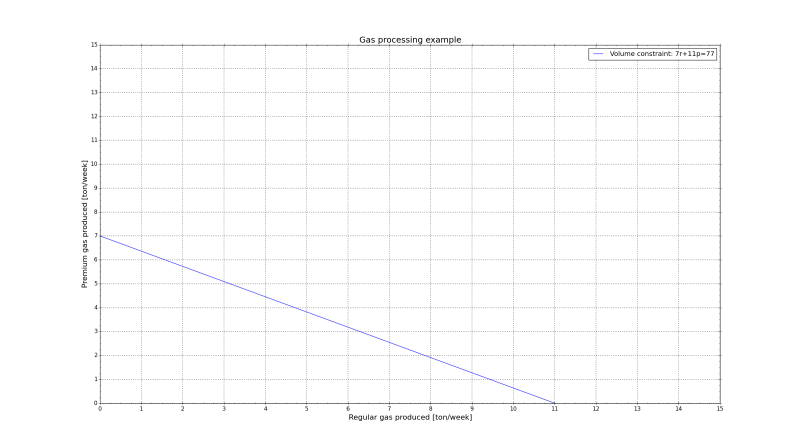
\includegraphics[width=0.95\textwidth]{gas.volume.jpg}
%       \caption{}
    \end{figure}
\end{frame}


\begin{frame}{}
    \begin{figure}
        \centering
        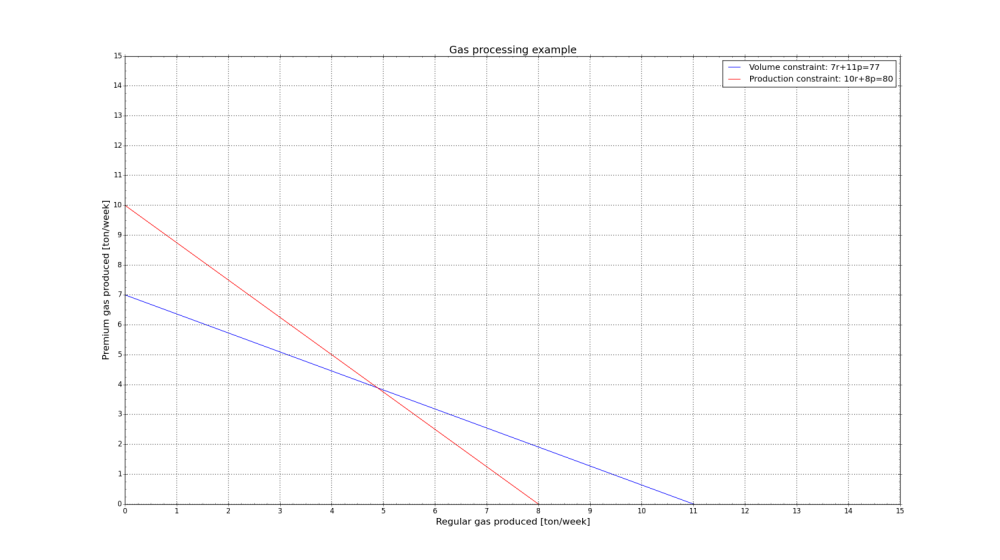
\includegraphics[width=0.95\textwidth]{gas.production.jpg}
%       \caption{}
    \end{figure}
\end{frame}


\begin{frame}{}
    \begin{figure}
        \centering
        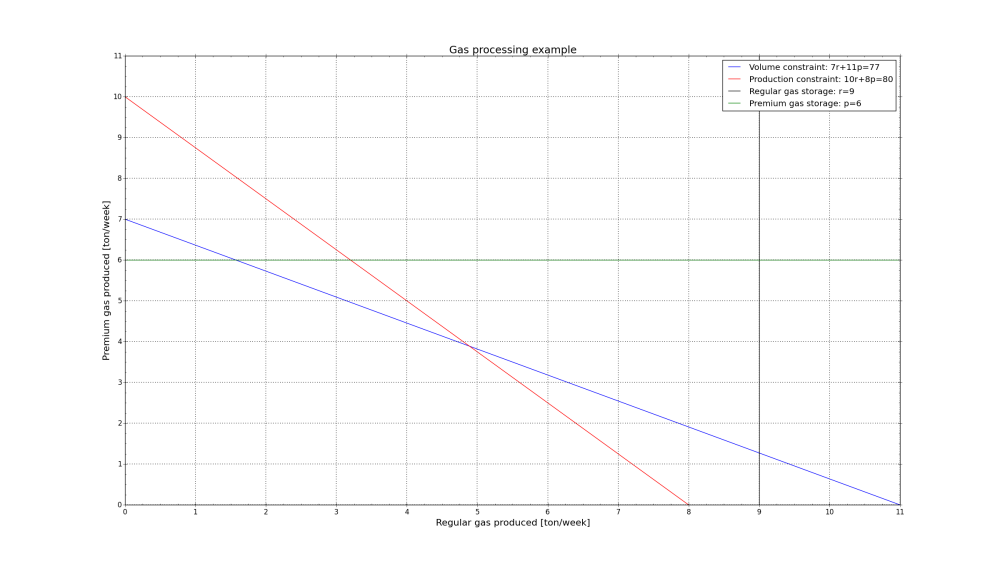
\includegraphics[width=0.95\textwidth]{gas.storage.jpg}
%       \caption{}
    \end{figure}
\end{frame}


\begin{frame}{Then maximize profit}
    \begin{enumerate}[series=outerlist,topsep=0pt,itemsep=1pt,leftmargin=*,label=(\arabic*)]
        \item[]Typically, it's a good idea to plot the 'break even' function --
    \end{enumerate}

    \vspace*{\fill}

    \begin{equation}
        \LARGE
        P = 150r +175p = 0
    \end{equation}

    \vspace*{\fill}

    \begin{enumerate}[series=outerlist,topsep=0pt,itemsep=1pt,leftmargin=*,label=(\arabic*)]
        \item[]Not in feasible space
            \vspace{0.05in}
        \item[]But we know the points of intersection bounding the feasible space
        \item[]$(0,0) - (0,6) - (1.7,6) - (4.9,3.9) - (0,8)$
    \end{enumerate}

    \begin{enumerate}[series=outerlist,topsep=9pt,itemsep=5pt,leftmargin=*,label=(\arabic*)]
        \item[]Substitute into the objective function --
        \item[]$P(0,0) = 0$
        \item[]$P(0,6) = 1050$
        \item[]$P(1.7,6) = 1305$
        \item[]$P(4.9,3.9) = 1418$ 
        \item[]$P(0,8) = 1400$
    \end{enumerate}
\end{frame}


\begin{frame}{}
    \begin{figure}
        \centering
        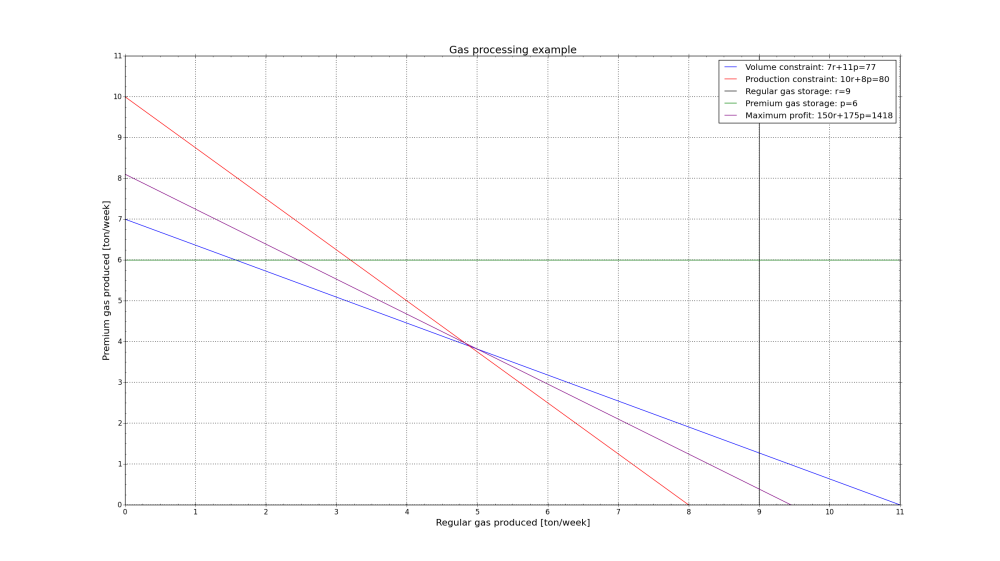
\includegraphics[width=0.95\textwidth]{gas.profit.jpg}
%       \caption{}
    \end{figure}
\end{frame}


\begin{frame}[plain]{}
    \centering\Large\textbf{Now for waste oxide loading}
\end{frame}


\addtocounter{framenumber}{-1} 
\begin{frame}{Apply to Japanese waste concept}
    \begin{enumerate}[series=outerlist,topsep=0pt,itemsep=3pt,leftmargin=*,label=(\arabic*)]
        \item[]\textbf{Objective function}
        \item[]We want to maximize the amount of waste oxide that can be loaded into an \acs{hlw} form of glass in a stainless steel canister
            \vspace{0.25in}
        \item[]\textbf{Decision variables}
        \item[]Waste Oxide Mass in the canister and Glass Oxide Mass in the canister
        \item[]$M_W, \; M_G$
    \end{enumerate}
\end{frame}


\begin{frame}[t]{}
    \begin{enumerate}[series=outerlist,topsep=0pt,itemsep=5pt,label=(\arabic*)]
        \item[]\textbf{Constraints}
        \item Total canister weight is 500 kg of waste mass + glass mass
        \item[]Include 100 kg for mass of the canister
            \vspace{0.15in}
        \item Volume of waste and glass is 0.15 cubic meters
            \vspace{0.15in}
        \item Empirical formula for volume constraint --
        \item[]$\rho = 1230r + 2419 \; \frac{kg}{m^3}$
        \item[]r = mass fraction of waste in the waste glass
            \vspace{0.15in}
        \item Heat generation limit is 2300 Watts
        \item[]$[C N_A \sum_i \frac{E_i \lambda_i x_i}{A_i}] \cdot M_W \leq 2300$
        \item[]This is tedious to find or compute all the data and not particularly constructive
        \item[]Just use 9.652
    \end{enumerate}
\end{frame}






























































































%\begin{frame}{}
%    \begin{equation}
%        \LARGE
%    \end{equation}
%
%    \begin{equation}
%        \LARGE
%    \end{equation}
%
%    \vspace*{\fill}
%
%    \begin{enumerate}[series=outerlist,topsep=0pt,itemsep=21pt,leftmargin=*,label=(\arabic*)]
%    \end{enumerate}
%
%    \vspace*{\fill}
%
%    \begin{equation}
%        \LARGE
%    \end{equation}
%
%    \vspace*{\fill}
%
%    \begin{enumerate}[series=outerlist,topsep=0pt,itemsep=21pt,leftmargin=*,label=(\arabic*)]
%    \end{enumerate}
%\end{frame}


%\begin{frame}{}
%    \begin{enumerate}[series=outerlist,topsep=0pt,itemsep=21pt,leftmargin=*,label=(\arabic*)]
%    \end{enumerate}
%
%    \vspace*{\fill}
%
%    \begin{equation}
%        \LARGE
%    \end{equation}
%
%    \vspace*{\fill}
%
%    \begin{enumerate}[series=outerlist,topsep=0pt,itemsep=11pt,leftmargin=*,label=(\arabic*)]
%    \end{enumerate}
%
%    \vspace*{\fill}
%
%    \begin{equation}
%        \LARGE
%    \end{equation}
%\end{frame}


%\begin{frame}{}
%    \begin{figure}
%        \centering
%        \includegraphics[width=0.85\textwidth]{}
%%       \caption{}
%    \end{figure}
%\end{frame}


































\begin{frame}[plain]{}
    \begin{figure}
        \centering
        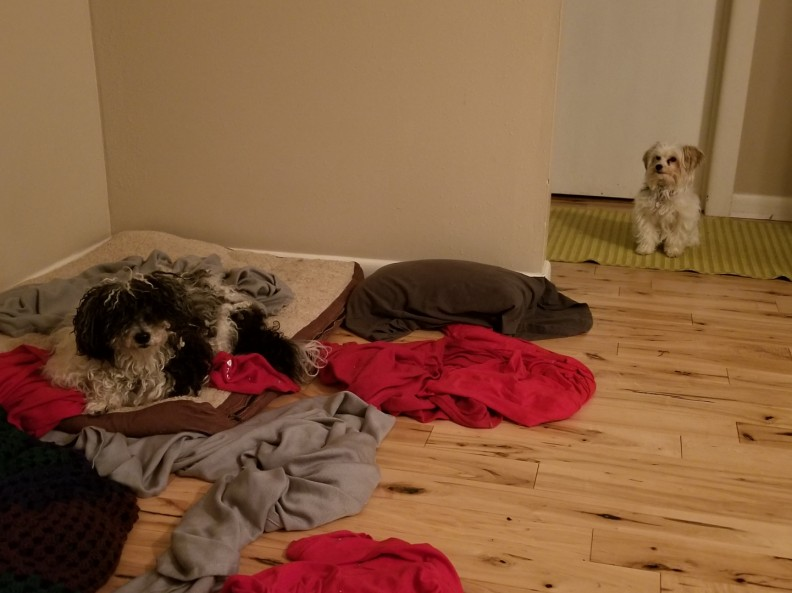
\includegraphics[width=0.75\textwidth]{final.jpg}
%        \caption{}
    \end{figure}
\end{frame}


%%%%%%%
%\begin{frame}{}
%    \begin{columns}
%
%        \begin{column}{0.50\textwidth}
%            \begin{enumerate}[series=outerlist,topsep=0pt,itemsep=21pt,leftmargin=*,label=(\arabic*)]
%                \item[]
%                \item[]
%            \end{enumerate}
%        \end{column}
%
%        \begin{column}{0.50\textwidth}
%            \begin{enumerate}[series=outerlist,topsep=0pt,itemsep=21pt,leftmargin=*,label=(\arabic*)]
%                \item[]
%                \item[]
%            \end{enumerate}
%        \end{column}
%
%    \end{columns}
%\end{frame}

%    \begin{figure}
%        \centering
%        \includegraphics[width=0.75\textwidth]{wsc.png}
%        \caption{\acs{wsc}}
%    \end{figure}


%\begin{frame}{References}
%    \bibliographystyle{nsf}
%    \footnotesize
%    \bibliography{references}
%\end{frame}
%%%%%%%


\end{document}
